\documentclass[a4paper,14pt,oneside]{extarticle}
% Thay doi chieu cao cua header va top margin
% de fix warning `\headheight is too small`
\setlength{\headheight}{17pt}
\addtolength{\topmargin}{-3pt}

% Package render ngon ngu tieng Viet
\usepackage[utf8]{vietnam}

% Package can le tren, duoi, trai, phai
\usepackage[left=3.5cm,right=2.5cm,top=2cm,bottom=2cm]{geometry}

% Packages de viet cong thuc Toan hoc
\usepackage{amsmath,amssymb, amsthm}
% Package de viet in dam cong thuc Toan hoc (bm = bold math)
\usepackage{bm}

% Package su dung de giu figure/table o dung vi tri
% \begin{figure}[H]
%     ... figure contents...
% \end{figure}
% Note: can check lai (comment ko thay khac biet)
\usepackage{float}

% Package de su dung duoc `subfigure`
\usepackage{subfigure}

% Package custom style cua caption
% (kich thuoc font chu, khoang cach so voi anh, ...)
\usepackage[font=small,skip=0pt]{caption}

% Package custom khoang cach
% giua cac gach dau dong trong danh sach
\usepackage{enumitem}
\setlist{nosep}

% Custom khoang cach giua cac dong (gian dong)
% Note: can check lai dong `usepackage` (comment ko thay khac biet)
\usepackage{setspace}
\renewcommand{\baselinestretch}{1.25}

% Package su dung font Times la font cho text va
% cung cap mot so syntax Toan hoc
\usepackage{mathptmx}

% Package su dung de reference/citation co the click
\usepackage{hyperref}

% Package su dung cho viec danh `chi muc tu khoa`
\usepackage{imakeidx}
\makeindex[columns=3, columnsep=0.5em, title=Chỉ mục từ khoá, intoc]

% Package su dung cho `khungtrangbia`
\usepackage{tikz}

% Package su dung cho `pythoncodestyle`
\usepackage{listings}

\usepackage{tocbasic}
\DeclareTOCStyleEntry[dynnumwidth=true, numsep=1em]{tocline}{section}
\renewcommand*{\thesection}{Chương \arabic{section}}
\renewcommand*{\thesubsection}{\arabic{section}.\arabic{subsection}}

% Package su dung cho `headerfooterstyle`
\usepackage{fancyhdr}

% Custom style cho header and footer
% De su dung duoc custom style nay, can `\usepackage{fancyhdr}`
\def\headerfooterstyle{
    \pagestyle{fancy}
    \fancyhf{}
    \lhead{Chương \thesection}
    \rhead{\thepage}
    \lfoot{}
    \rfoot{Nguyễn Hữu Minh}
    \renewcommand{\headrulewidth}{2pt}
    \renewcommand{\footrulewidth}{1pt}
}

\headerfooterstyle

% Package su dung de ve bang `tab_result` trong file `4_munit_results.tex`
\usepackage[flushleft]{threeparttable}

% Package su dung de dung `tab` \tab
\usepackage{tabto}

% Khai bao ky tu unicode de sua error
% Package inputenc: Unicode character − (U+2212) (inputenc) not set up for use with LaTeX.
\DeclareUnicodeCharacter{2212}{-}

\begin{document}

    % BAT DAU CAC TRANG CHUC NANG
    % Xoa page number
    \pagenumbering{gobble}
    % Xoa header - footer
    \pagestyle{plain}

    
\def\trangbia{
    % % De dung "khung_trang_bia", ta can `\usepackage{tikz}`
    % 
% De su dung "khungtrangbia", ta can `\usepackage{tikz}`
\def\khungtrangbia{
  \begin{tikzpicture}[remember picture,overlay,inner sep=0,outer sep=0]
    \draw[black!70!black,line width=3pt]([xshift=-2cm,yshift=-2.5cm]current page.north east)
    coordinate (A) -- ([xshift=2.5cm,yshift=-2.5cm]current page.north west)
    coordinate (B) -- ([xshift=2.5cm,yshift=2.5cm]current page.south west)
    coordinate (C) -- ([xshift=-2cm,yshift=2.5cm]current page.south east)
    coordinate (D) -- cycle;
    \draw ([yshift=0.5cm,xshift=-0.5cm]A) --
    ([yshift=0.5cm,xshift=0.5cm]B) --
    ([yshift=-0.5cm,xshift=0.5cm]B) --
    ([yshift=-0.5cm,xshift=-0.5cm]B) --
    ([yshift=0.5cm,xshift=-0.5cm]C) --
    ([yshift=0.5cm,xshift=0.5cm]C) --
    ([yshift=-0.5cm,xshift=0.5cm]C) --
    ([yshift=-0.5cm,xshift=-0.5cm]D) --
    ([yshift=0.5cm,xshift=-0.5cm]D) --
    ([yshift=0.5cm,xshift=0.5cm]D) --
    ([yshift=-0.5cm,xshift=0.5cm]A) --
    ([yshift=-0.5cm,xshift=-0.5cm]A) --
    ([yshift=0.5cm,xshift=-0.5cm]A);
    \draw ([yshift=-0.3cm,xshift=0.3cm]A) --
    ([yshift=-0.3cm,xshift=-0.3cm]B) --
    ([yshift=0.3cm,xshift=-0.3cm]B) --
    ([yshift=0.3cm,xshift=0.3cm]B) --
    ([yshift=-0.3cm,xshift=0.3cm]C) --
    ([yshift=-0.3cm,xshift=-0.3cm]C) --
    ([yshift=0.3cm,xshift=-0.3cm]C) --
    ([yshift=0.3cm,xshift=0.3cm]D) --
    ([yshift=-0.3cm,xshift=0.3cm]D) --
    ([yshift=-0.3cm,xshift=-0.3cm]D) --
    ([yshift=0.3cm,xshift=-0.3cm]A) --
    ([yshift=0.3cm,xshift=0.3cm]A) --
    ([yshift=-0.3cm,xshift=0.3cm]A);
  \end{tikzpicture}
}

    % \vekhungtrangbia
    
    \large {\bf \centerline {TRƯỜNG ĐẠI HỌC BÁCH KHOA HÀ NỘI}}
    \vskip 2in

    % \begin{center}
    %     \includegraphics[width=0.25\columnwidth]{images/logo_bk.png}
    % \end{center}
    % \vskip 0.5in

    \LARGE {\bf \centerline {LUẬN VĂN THẠC SĨ}}
    \vskip 0.3in

    \LARGE {\bf \centerline {Ứng dụng các mô hình học sâu}}
    \LARGE {\bf \centerline {giải quyết một số bài toán}}
    \LARGE {\bf \centerline {phân tích và xử lý hình ảnh}}
    \vskip 0.3in

    \normalsize {\bf \centerline {NGUYỄN HỮU MINH}}
    \vskip 0in
    \normalsize {\centerline {Minh.NH202955M@sis.hust.edu.vn}}
    \vskip 0.1in
    \normalsize {\centerline {\textbf{Ngành}: Toán Tin}}
    \vskip 0in
    \normalsize {\centerline {\textbf{Chuyên ngành}: Toán Tin}}
    \vskip 1.3in

    \hspace{0.5cm}
    \small {\textbf{Giảng viên hướng dẫn}: TS. Bùi Xuân Diệu}
    \hspace{0.5cm}
    \begin{tikzpicture}
        \draw (15.5,0)--(18.5,0);
    \end{tikzpicture}
    \vskip 0in

    \hspace{0.5cm}
    \small {\textbf{Bộ môn}: Toán cơ bản \hspace{4.2cm} Chữ ký của GVHD}
    \vskip 0in

    \hspace{0.5cm}
    \small {\textbf{Viện}: Toán ứng dụng và Tin học}
    \vskip 1.5in
  
    \small {\centerline{\textbf{HÀ NỘI, 08/2022}}}
}

    \trangbia

    \newpage
    
\def\loicamon{
    \section*{Lời cảm ơn}
    \addcontentsline{toc}{section}{Lời cảm ơn}
    Thành công nào cũng đều gắn liền với sự hỗ trợ của những người xung quanh, dù cho là ít hay nhiều, trực tiếp hay gián tiếp. Trong suốt thời gian làm Đồ án, em đã nhận được sự quan tâm, giúp đỡ của thầy cô, gia đình, anh chị và bạn bè xung quanh.\\
    Với tấm lòng biết ơn vô cùng sâu sắc, em xin gửi lời cảm ơn chân thành nhất từ đáy lòng đến quý Thầy Cô của Viện Toán ứng dụng và Tin học, trường Đại học Bách Khoa Hà Nội đã tạo điều kiện và cùng dùng những tri thức, tâm huyết của mình để có thể truyền đạt cho em trong vốn kiến thức quý báu. \\
    Đặc biệt, em xin chân thành cảm ơn ThS. Nguyễn Tuấn Dũng đã tận tâm chỉ bảo hướng dẫn em trong suốt thời gian làm Đồ án qua. Nhờ có những lời hướng dẫn, dạy bảo của thầy mà Đồ án của em đã hoàn thành một cách tốt nhất. Một lần nữa, em xin gửi lời cảm ơn chân thành đến thầy. \\
    Đồ án của em không tránh khỏi những thiếu sót, em rất mong nhận được ý kiến đóng góp của quý Thầy Cô và các bạn học để Đồ án của em được hoàn thiện hơn. \\
    Em xin chân thành cảm ơn!
}

    \loicamon
    
\def \tomtatnoidung{
    \section*{Tóm tắt nội dung đồ án}
    \addcontentsline{toc}{section}{Tóm tắt nội dung đồ án}
    Cách mạng công nghiệp 4.0 đã mang đến cho con người một kỷ nguyên khai phá dữ liệu. Điều này đặt ra bài toán không chỉ làm sao để khai phá được dữ liệu một cách hiệu quả mà còn làm sao để sinh ra được thêm nhiều dữ liệu một cách tự động và với số lượng lớn. Do đó, trong khuôn khổ của đồ án tốt nghiệp, em sẽ nghiên cứu về ý tưởng chung, kiến trúc, hàm loss, phương pháp đánh giá, những vấn đề tồn đọng và cách giải quyết các vấn đề đó của mô hình Generative Adversarial Networks (GANs) tổng quát nhằm giải quyết bài toán sinh dữ liệu ảnh nói và mô hình Multimodal Unsupervised Image-to-Image Translation (MUNIT) giúp giải quyết bài toán sinh dữ liệu ảnh mới từ ảnh đã có sẵn (Image-to-Image Translation). Bên cạnh những kết quả đã được công bố trong bài báo, em đã thử nghiệm mô hình với bộ dữ liệu khác để chứng minh tính đúng đắn của mô hình và lấy đó làm tiền đề cho việc phát triển những mô hình phức tạp hơn trong tương lai.
    \vskip 2.5in

    \hspace{7.7cm}
    \normalsize {Hà Nội, ngày \hspace{0.5cm} tháng \hspace{0.5cm} năm}
    \vskip 0in

    \hspace{8.5cm}
    \normalsize {\textit{Sinh viên thực hiện}}
}
    \tomtatnoidung

    % Bat dau danh so trang page number
    \pagenumbering{arabic}

    \newpage
    \tableofcontents

    \newpage
    \listoffigures
    \addcontentsline{toc}{section}{Danh sách hình vẽ}

    % KET THUC CAC TRANG CHUC NANG

    % BAT DAU PHAN NOI DUNG CHINH
    \newpage
    \def\problems{
    \section*{Phát biểu các bài toán}
    \addcontentsline{toc}{section}{Phát biểu các bài toán}
    \subsection*{Bài toán nhận diện đối tượng\index{nhận diện đối tượng}}
    Bài toán nhận diện đối tượng\index{nhận diện đối tượng} (object detection\index{object detection}) là một bài toán rất phổ biến trong lĩnh vực thị giác máy tính và được coi là một trong số các bài toán máy học kinh điển.
    Một số ứng dụng của bài toán như: trong y tế giúp nhận diện vị trí bị bệnh trong cơ thể, trong bảo mật giúp định nhận diện con người trong khu vực cấm, trong nông nghiệp giúp xác định số lượng nông sản.

    \noindent
    Bài toán nhận diện đối tượng\index{nhận diện đối tượng} là sự tổng hợp của hai bài toán con: bài toán định vị đối tượng\index{định vị đối tượng} (object localization\index{object localization}) và bài toán phân loại ảnh\index{phân loại ảnh} (image classification\index{image classification}).
    Cụ thể hơn, bài toán định vị đối tượng là bài toán xác định vị trí của đối tượng trong ảnh bằng các hộp giới hạn\index{hộp giới hạn} (bounding box\index{bounding box}) đại diện cho vị trí của từng đối tượng.
    Trong khi đó, bài toán phân loại ảnh\index{bài toán phân loại ảnh} giúp xác định đối tượng vừa được định vị là đối tượng nào.

    \noindent
    Với sự quan tâm của giới nghiên cứu cho bài toán nhận diện đối tượng\index{nhận diện đối tượng}, đã có rất nhiều các nghiên cứu và giải pháp ra đời đạt được độ chính xác cao và chạy trong thời gian thực.

    \subsection*{Bài toán nhận diện khuôn mặt}
    Bài toán nhận diện khuôn mặt\index{nhận diện khuôn mặt} (face detection\index{face detection}) là một bài toán nền tảng cực kỳ quan trọng cho rất nhiều các bài toán khác về khuôn mặt như xác thực khuôn mặt, sinh ra ảnh khuôn mặt, phân lớp các thuộc tính trên khuôn mặt.
    Những ứng dụng của nhóm bài toán liên quan đến khuôn mặt có thể kể đến như nhận diện khách hàng, điểm danh chấm công, phân tích cảm xúc.
    Với những tiềm năng trên, nhận diện khuôn mặt trở thành một nhánh nghiên cứu thu hút rất nhiều sự quan tâm của giới nghiên cứu vì tính ứng dụng cao và động lực đẩy độ chính xác của mô hình giải bài toán này lên đến tuyệt đối.
    
    \noindent
    Nhiều nghiên cứu đã nhấn mạnh vào những đặc thù riêng biệt của khuôn mặt con người so với đối tượng sự vật nói chung để đưa ra những giải pháp nhằm thúc đẩy độ chính xác của mô hình.
    Tuy vậy, trong nghiên cứu \cite{zhu2020tinaface}, nhóm tác giả đã chỉ ra rằng nhận diện khuôn mặt vẫn chỉ là một bài toán con của bài toán nhận diện đối tượng\index{nhận diện đối tượng} và vẫn có thể được giải một cách hiệu quả bằng các mô hình nhận diện đối tượng\index{nhận diện đối tượng} nói chung.

    \subsection*{Bài toán nhận diện khuôn mặt với ảnh chất lượng cao}
    Mặc dù đã có nhiều các nghiên cứu quan tâm đến bài toán nhận diện đối tượng\index{nhận diện đối tượng} và nhận diện khuôn mặt, nhưng vẫn tồn tại vấn đề nan giải là bài toán nhận diện đối với ảnh chất lượng cao được chụp từ những camera hiện đại.
    Việc xử lý những hình ảnh có kích thước lớn như 4K (3840×2160) hay 8K (7680×4320) bằng các mô hình học sâu gây ra nhiều vấn đề về chi phí và thời gian tính toán.
    Do đó, việc sử dụng những hình ảnh chất lượng cao trong quá trình dự đoán đã khó, việc huấn luyện mô hình với những hình ảnh này gần như bất khả thi.

    \noindent
    Một cách đơn giản là thu nhỏ kích thước ảnh trước khi đưa vào mô hình học sâu.
    Tuy nhiên cách làm này gây ra việc mất mát rất nhiều thông tin của các đối tượng ở trên ảnh, đặc biệt đối với các đối tượng có kích thước nhỏ.
    Sau khi thu nhỏ ảnh ban đầu, những đối tượng này gần như biến mất khỏi ảnh và gây ra khó khăn cho mô hình để có thể thu thập được các đặc trưng của các đối tượng này.
    Vì vậy, ta cần giải pháp tốt hơn để xử lý ảnh chất lượng cao, sao cho vừa đảm bảo về độ chính xác vừa đảm bảo về chi phí và thời gian tính toán của mô hình.
}
    \problems
    
    % Bat dau hien header - footer tu trang nay ve sau
    \newpage
    \pagestyle{fancy}
    \def\theory{
    \section{Cơ sở lý thuyết}
    Các nghiên cứu hiện đại nhất về việc giải quyết bài toán nhận diện khuôn mặt và nhận diện khuôn mặt trong ảnh chất lượng cao kế thừa rất nhiều ý tưởng từ các nghiên cứu giải quyết bài toán nhận diện đối tượng\index{nhận diện đối tượng}.

    \noindent
    Các mô hình giải quyết bài toán nhận diện đối tượng\index{nhận diện đối tượng} được chia thành hai nhóm: nhóm các mô hình hai pha\index{hai pha} (two-stage\index{two-stage}) và nhóm các mô hình một pha\index{một pha} (single-stage\index{single-stage}).
    Các mô hình hai pha\index{hai pha} phổ biến là R-CNN \cite{girshick2014rich}, Fast R-CNN \cite{girshick2015fast}, Faster R-CNN \cite{ren2015faster} và FPN \cite{lin2017feature}.
    Các mô hình hai pha\index{hai pha} này đạt độ chính xác rất cao, tuy nhiên, tốc độ chạy không thật sự nhanh và đây là động lực để các mô hình một pha\index{một pha} ra đời. 
    Các mô hình một pha\index{một pha} nổi tiếng và thu hút nhiều sự quan tâm như SSD \cite{liu2016ssd}, chuỗi các mô hình YOLO \cite{redmon2016look, redmon2016yolo9000, redmon2018yolov3, bochkovskiy2020yolov4}, RetinaNet \cite{lin2017focal}.

    \noindent
    Bên cạnh đó, nhiều nghiên cứu trong những năm gần đây đã tập trung vào việc xử lý ảnh chất lượng cao.
    Các mô hình này hướng tới việc duy trì và tăng cường độ chính xác của mô hình nhận diện đối tượng\index{nhận diện đối tượng} và tiết kiệm tối đa chi phí tính toán.
    Một số nghiên cứu đáng chú ý như SNIP \cite{singh2018analysis}, SNIPER\index{SNIPER} \cite{singh2018sniper}, Scale Match \cite{yu2020scale} hướng đến quá trình huấn luyện của mô hình với ảnh chất lượng cao, AutoFocus \cite{najibi2019autofocus}, Attention pipeline \cite{ruuvzivcka2018fast}, Dynamic Zoom-in \cite{gao2018dynamic}, PeleeNet \cite{ozge2019power} đưa ra các ý tưởng cải thiện quá trình dự đoán của mô hình với ảnh chất lượng cao.

    \noindent
    Lấy nền tảng từ các mô hình nhận diện đối tượng\index{nhận diện đối tượng}, các mô hình nhận diện khuôn mặt bổ sung hoặc chỉnh sửa một số điểm nhằm tăng độ chính xác trên các bộ dữ liệu về khuôn mặt.
    Dựa trên SSD \cite{liu2016ssd}, mô hình S3FD \cite{zhang2017s3fd} thay đổi chiến lược sinh khu vực mỏ neo\index{khu vực mỏ neo} nhằm đạt độ chính xác cao hơn trên dữ liệu khuôn mặt.
    Mô hình Pyramid Box \cite{tang2018pyramidbox} và Pyramid Box++ \cite{li2019pyramidbox++} thay đổi kiến trúc của mô hình FPN \cite{lin2017feature} phù hợp hơn đối với bài toán nhận diện khuôn mặt.
    Hay mô hình RetinaFace \cite{deng2020retinaface}, kế thừa từ RetinaNet \cite{lin2017focal}, sử dụng thêm dữ liệu và hàm mất mát đặc trưng của khuôn mặt.

    \subsection{Mô hình Faster R-CNN}
    \def\fasterrcnn{
    Được lấy động lực từ những điểm yếu của mô hình R-CNN \cite{girshick2014rich} và Fast R-CNN \cite{girshick2015fast}, nhóm tác giả đã nghiên cứu và phát triển mô hình Faster R-CNN \cite{ren2015faster} với trung tâm là kiến trúc mô hình Region Proposal Network (gọi tắt là RPN).
    Mô hình RPN được kỳ vọng sẽ thay thế hoàn toàn các thuật toán như Selective Search \cite{uijlings2013selective} trong kiến trúc của các mô hình two-stage giải quyết bài toán nhận diện đối tượng, hướng đến việc cải thiện không chỉ tốc độ của mô hình mà còn cải thiện về độ chính xác.

    \subsubsection*{Kiến trúc mô hình RPN}
    Mô hình RPN nhận đầu vào là ảnh với kích thước bất kỳ và trả đầu ra là toạ độ của các khu vực và xác suất khu vực đó là đối tượng nào trong các lớp đối tượng\index{lớp đối tượng}.
    Nhằm tiết kiệm chi phí tính toán, mô hình RPN dùng chung phần mô hình xương sống\index{mô hình xương sống} với Fast R-CNN.

    \begin{figure}[H]
        \centering
        \includegraphics[width=9cm] {images/faster_rcnn_rpn}
        \caption{Kiến trúc mô hình RPN (Nguồn: \cite{ren2015faster})}
        \label{fig:faster_rcnn_rpn}
    \end{figure}
    
    \noindent
    Sau khi đưa ảnh qua mô hình xương sống\index{mô hình xương sống} và thu được một bản đồ đặc trưng\index{bản đồ đặc trưng}, mô hình RPN nhận đầu vào là bản đồ đặc trưng\index{bản đồ đặc trưng} này và trả đầu ra là các khu vực đề xuất gọi là các khu vực mỏ neo\index{khu vực mỏ neo}.
    Nhóm tác giả xây dựng phương pháp đề xuất các khu vực mỏ neo\index{khu vực mỏ neo} dựa trên kích thước và tỷ lệ giữa chiều dài và chiều rộng của khu vực mỏ neo\index{khu vực mỏ neo}.
    Cụ thể, mô hình RPN đưa bản đồ đặc trưng\index{bản đồ đặc trưng} qua một lớp Conv\index{lớp Conv} và thu được một bản đồ đặc trưng\index{bản đồ đặc trưng} mới có kích thước W x H.
    Từ đó, nhóm tác giả đề xuất ba kích thước của khu vực mỏ neo\index{khu vực mỏ neo} và ba tỷ lệ giữa chiều dài và chiều rộng của khu vực mỏ neo\index{khu vực mỏ neo} tạo ra chín khu vực mỏ neo\index{khu vực mỏ neo} với mỗi điểm ảnh\index{điểm ảnh} trên bản đồ đặc trưng\index{bản đồ đặc trưng} kích thước W x H.
    Tổng cộng trên toàn bộ bản đồ đặc trưng\index{bản đồ đặc trưng} kích thước W x H, ta thu được W x H x 9 khu vực mỏ neo\index{khu vực mỏ neo}.
    Các bản đồ đặc trưng\index{bản đồ đặc trưng} đại diện cho các khu vực mỏ neo\index{khu vực mỏ neo} này được tiếp tục đưa qua các lớp Conv\index{lớp Conv} để biến đổi về các bản đồ đặc trưng\index{bản đồ đặc trưng} mới có dạng (W x H x 9) x 1 đại diện cho xác suất khu vực mỏ neo\index{khu vực mỏ neo} đó là đối tượng và có dạng (W x H x 9) x 4 đại diện cho 4 toạ độ x của góc trái trên, y của góc trái trên, chiều dài và chiều rộng của hộp giới hạn\index{hộp giới hạn}.

    \noindent
    Một điểm mạnh của RPN so với các mô hình nhận diện đối tượng thời bấy giờ đó chính là khả năng dự đoán được các đối tượng có kích thước khác nhau và tỷ lệ giữa chiều dài và chiều rộng khác nhau nhờ vào cách cấu hình của khu vực mỏ neo\index{khu vực mỏ neo}.

    \begin{figure}[H]
        \centering
        \includegraphics[width=15cm] {images/faster_rcnn_multi_scale_anchor}
        \caption{So sánh các kiến trúc xử lý vấn đề đối tượng có kích thước khác nhau và tỷ lệ giữa chiều dài và chiều rộng khác nhau (Nguồn: \cite{ren2015faster})}
        \label{fig:faster_rcnn_multi_scale_anchor}
    \end{figure}

    \noindent
    Một số kiến trúc đã được đề xuất ở thời điểm đó nhưng đều gặp phải rào cản về khối lượng tính toán lớn. \\
    - Kiến trúc đầu tiên là \textit{image / feature pyramids} sử dụng ảnh với nhiều kích thước khác nhau nhằm tạo ra bản đồ đặc trưng\index{bản đồ đặc trưng} có nhiều kích thước khác nhau.
    Kiến trúc này tốn rất nhiều chi phí tính toán do ta cần xử lý nhiều lần (thường là ba lần) với mỗi ảnh đầu vào khác nhau. \\
    - Kiến trúc thứ hai là \textit{pyramid of filters} đưa cùng một bản đồ đặc trưng\index{bản đồ đặc trưng} đầu vào qua nhiều khối Conv có kích thước của kernel khác nhau (thường là Conv với có kích thước 5x7 và Conv với có kích thước 7x5).
    Kiến trúc này tiết kiệm chi phí tính toán hơn một chút so với kiến trúc đầu tiên và thường được sử dụng kết hợp cùng với kiến trúc đầu tiên. \\
    - Kiến trúc cuối cùng là \textit{pyramid of anchors} được đề xuất trong RPN sử dụng nhiều khu vực mỏ neo\index{khu vực mỏ neo} với các kích thước khác nhau và tỷ lệ giữa chiều dài và chiều rộng khác nhau.
    Kiến trúc này chỉ tăng một lượng nhỏ chi phí tính toán nếu ta tăng số lượng khu vực mỏ neo\index{khu vực mỏ neo}, còn phần chi phí tính toán đối với bản đồ đặc trưng\index{bản đồ đặc trưng} vẫn được giữ nguyên. \\
    Phần cải tiến của RPN đối với đối tượng có kích thước khác nhau và tỷ lệ giữa chiều dài và chiều rộng khác nhau chỉ là những cải tiến tại thời điểm đó mà thôi.

    \subsubsection*{Hàm mất mát và cách huấn luyện mô hình RPN}
    Để huấn luyện được mô hình RPN, nhóm tác giả gán cho mỗi khu vực mỏ neo\index{khu vực mỏ neo} một lớp groundtruth\index{groundtruth} và thiết lập hàm mất mát\index{hàm mất mát} đối với từng khu vực mỏ neo\index{khu vực mỏ neo}.
    Nhóm tác giả gán lớp groundtruth\index{groundtruth} dương cho khu vực mỏ neo\index{khu vực mỏ neo} dựa theo hai cách sau: \\
    - Những khu vực mỏ neo\index{khu vực mỏ neo} có chỉ số IoU\index{IoU} lớn nhất đối với một groundtruth\index{groundtruth} hộp giới hạn\index{hộp giới hạn} được gán là khu vực mỏ neo\index{khu vực mỏ neo} dương. \\
    - Những khu vực mỏ neo\index{khu vực mỏ neo} có chỉ số IoU\index{IoU} lớn hơn 0.7 đối với một groundtruth\index{groundtruth} hộp giới hạn\index{hộp giới hạn} được gán là khu vực mỏ neo\index{khu vực mỏ neo} dương. \\
    Với hai cách như trên, một groundtruth\index{groundtruth} hộp giới hạn\index{hộp giới hạn} có thể gán được cho nhiều khu vực mỏ neo\index{khu vực mỏ neo} khác nhau.
    Ngoài ra, nhóm tác giả cũng gán lớp groundtruth\index{groundtruth} âm cho các khu vực mỏ neo\index{khu vực mỏ neo} không phải là dương và có chỉ số IoU\index{IoU} nhỏ hơn 0.3 đối với một groundtruth\index{groundtruth} hộp giới hạn\index{hộp giới hạn}. \\
    Từ đó, mô hình Faster R-CNN tối ưu hàm mất mát\index{hàm mất mát} sau:

    \begin{equation}
        \label{eq:faster_rcnn_loss}
        L(\{p_i\}, \{t_i\}) = \frac{1}{N_{cls}}\sum_i L_{cls}(p_i, p^{*}_i) + \lambda\frac{1}{N_{reg}}\sum_i  p^{*}_i L_{reg}(t_i, t^{*}_i).
    \end{equation}

    \noindent
    trong đó: \\
    - \textit{i} là chỉ số của từng khu vực mỏ neo\index{khu vực mỏ neo}. \\
    - \textit{$p_i$} là xác suất mà khu vực mỏ neo\index{khu vực mỏ neo} chứa đối tượng. \\
    - \textit{$p^{*}_i$} là groundtruth\index{groundtruth} của khu vực mỏ neo\index{khu vực mỏ neo} (là 1 nếu khu vực mỏ neo\index{khu vực mỏ neo} đó được gán là chứa đối tượng, là 0 nếu khu vực mỏ neo\index{khu vực mỏ neo} đó được gán là không chứa đối tượng). \\
    - \textit{$t_i$} là vector gồm 4 giá trị đại diện cho toạ độ của khu vực mà mô hình RPN đề xuất. \\
    - \textit{$t^{*}_i$} là vector gồm 4 giá trị đại diện cho toạ độ của groundtruth\index{groundtruth} hộp giới hạn\index{hộp giới hạn} tương ứng với khu vực mỏ neo\index{khu vực mỏ neo} đó. \\
    Hàm mất mát\index{hàm mất mát} trên gồm các thành phần: \\
    - \textit{$L_{cls}$}: là hàm mất mát\index{hàm mất mát} phân lớp thông thường giúp xác định khu vực mỏ neo\index{khu vực mỏ neo} có chứa đối tượng hay không. \\
    - \textit{$L_{reg}$}: là hàm mất mát\index{hàm mất mát} hồi quy đối với các khu vực mỏ neo\index{khu vực mỏ neo} dương, giúp tinh chỉnh toạ độ của khu vực mà mô hình đề xuất.
    Cụ thể, nhóm tác giả sử dụng $L_{reg}(t_i, t^{*}_i)=L_1(t_i - t^{*}_i)$ giống với hàm mất mát\index{hàm mất mát} sử dụng trong mô hình Fast R-CNN \cite{girshick2015fast}.

    \noindent
    Mô hình RPN được thiết kế để có thể huấn luyện cùng với quá trình huấn luyện nhận diện đối tượng từ đó giúp kết quả đề xuất khu vực trở nên chính xác hơn.
    Tuy nhiên, có một vấn đề nảy sinh khi sử dụng mô hình RPN cho việc đề xuất khu vực, đó là mô hình sẽ đề xuất ra nhiều các khu vực mỏ neo\index{khu vực mỏ neo} âm hơn rất nhiều so với số khu vực mỏ neo\index{khu vực mỏ neo} dương.
    Việc huấn luyện mô hình trên từng khu vực mỏ neo\index{khu vực mỏ neo} kết hợp với hiện tượng trên sẽ khiến cho tổng quan mô hình nhận diện đối tượng bị mất cân bằng dữ liệu\index{mất cân bằng dữ liệu}.
    Ngoài ra, việc huấn luyện mô hình với toàn bộ số khu vực mỏ neo\index{khu vực mỏ neo} được đề xuất ra cũng sẽ khiến cho khối lượng tính toán lớn và thời gian kéo dài quá trình huấn luyện mô hình.
    Từ đó, nhóm tác giả đề xuất việc lựa chọn ngẫu nhiên 256 khu vực mỏ neo\index{khu vực mỏ neo} trên mỗi ảnh để thực hiện việc tính giá trị hàm mất mát\index{hàm mất mát}. Việc lựa chọn này giúp tỷ lệ khu vực mỏ neo\index{khu vực mỏ neo} dương và âm trở nên cân bằng hơn và giảm thiểu bởi những phần khối lượng tính toán dư thừa.

    \subsubsection*{Sự kết hợp giữa mô hình RPN và Fast R-CNN}
    Nhóm tác giả cho rằng, việc huấn luyện mô hình RPN và Fast R-CNN cần phải diễn ra đồng thời, vì từ đó, việc chia sẻ chung thành phần mô hình xương sống\index{mô hình xương sống} Conv mới trở nên hiệu quả.

    \begin{figure}[H]
        \centering
        \includegraphics[width=8cm] {images/faster_rcnn_model}
        \caption{Toàn cảnh sự kết hợp của mô hình RPN và Fast R-CNN tạo ra mô hình Faster R-CNN (Nguồn: \cite{ren2015faster})}
        \label{fig:faster_model}
    \end{figure}

    \noindent
    Nhóm tác giả nêu ra ba phương án để huấn luyện mô hình RPN kết hợp với Fast R-CNN: \\
    - Cách 1: \textit{Alternating training}: Nhóm tác giả huấn luyện mô hình RPN trước sử dụng những hàm mất mát\index{hàm mất mát} của RPN nói trên.
    Sau khi huấn luyện xong mô hình RPN, tác giả sử dụng những khu vực được đề xuất bởi RPN để huấn luyện mô hình Fast R-CNN.
    Mô hình xương sống\index{mô hình xương sống} sau khi được huấn luyện bởi Fast R-CNN tiếp tục được sử dụng để huấn luyện mô hình RPN mới và vòng lặp này tiếp tục diễn ra cho đến khi kết quả của mô hình hội tụ. \\
    - Cách 2: \textit{Approximate joint training}: Phương pháp này kết hợp RPN và Fast R-CNN thành một mô hình duy nhất trong quá trình huấn luyện.
    Các khu vực được đề xuất bởi RPN được coi như là tất định đối với nhánh Fast R-CNN và khiến cho phương pháp huấn luyện này được gọi là \textit{approximate} bởi vì những thông tin từ nhánh Fast R-CNN sẽ không được cập nhật cho nhánh RPN.
    Quá trình lan truyền ngược\index{lan truyền ngược} được thực hiện độc lập giữa RPN và Fast R-CNN, riêng phần mô hình xương sống\index{mô hình xương sống} chung của RPN và Fast R-CNN được cập nhật theo giá trị hàm mất mát\index{hàm mất mát} của cả RPN và Fast R-CNN.
    Phương pháp này đạt hiệu quả thấp hơn chút so với \textit{Alternating training} tuy nhiên thời gian huấn luyện được giảm 25 - 50\%. \\
    - Cách 3: \textit{Non-approximate joint training}: Phương pháp này cải thiện được vấn đề \textit{approximate} tồn đọng của \textit{Approximate joint training}.
    Tuy nhiên, để làm được điều này, nhóm tác giả cần tinh chỉnh lại lớp RoI pooling trong Fast R-CNN để có thể update cho cả các thành phần của mô hình Fast R-CNN và RPN.
    Điều này nằm ngoài nội dung của nghiên cứu này nên nhóm tác giả không đề cập kỹ hơn.

    \noindent
    Tóm lại, nhóm tác giả dựa vào phương pháp \textit{Alternating training} và thực hiện quá trình huấn luyện gồm bốn bước như sau: \\
    - Bước 1: Nhóm tác giả khởi tạo mô hình RPN với pretrained ImageNet và huấn luyện mô hình RPN. \\
    - Bước 2: Nhóm tác giả khởi tạo mô hình Fast R-CNN với pretrained ImageNet và huấn luyện mô hình Fast R-CNN với các khu vực được đề xuất bởi RPN. \\
    - Bước 3: Nhóm tác giả khởi tạo lại mô hình RPN nhưng sử dụng phần mô hình xương sống\index{mô hình xương sống} đã được huấn luyện từ Bước 2.
    Nhóm tác giả chỉ huấn luyện những lớp riêng của mô hình RPN và không cập nhật cho phần mô hình xương sống\index{mô hình xương sống}. \\
    - Bước 4: Nhóm tác giả finetune lại những lớp riêng của mô hình Fast R-CNN với các khu vực được đề xuất bởi RPN và thu được mô hình Faster R-CNN cuối cùng. \\
    Nhóm tác giả cũng đã lặp lại bốn bước trên vài lần nhưng kết quả không thay đổi quá nhiều.

    \subsubsection*{Vấn đề tồn đọng của mô hình Faster R-CNN}
    Kết quả của mô hình Faster R-CNN và tâm điểm là kiến trúc RPN giúp thay thế thuật toán Selective Search đã giúp cho Faster R-CNN đạt độ chính xác cao hơn so với mô hình Fast R-CNN sử dụng Selective Search.
    Hơn nữa, RPN giúp cho Faster R-CNN nhanh hơn tới 10 lần so với cấu hình tương tự Fast R-CNN sử dụng Selective Search.
    Điều này giúp cho Faster R-CNN cho đến nay vẫn là một mô hình tốt để giải quyết bài toán nhận diện đối tượng, vừa đạt độ chính xác cao, vừa có tốc độ tương đối tốt.
    Tuy nhiên, cho đến thời điểm thực hiện luận văn này, đã có nhiều mô hình khác hiện đại hơn chỉ ra những vấn đề tồn đọng của Faster R-CNN như độ chính xác cần phải cải thiện thêm hay tốc độ chưa đạt đến ngưỡng chạy trong thời gian thực. 
}
    \fasterrcnn

    \subsection{Kiến trúc Feature Pyramid Networks}
    \def\fpn{
    Các kiến trúc mô hình xương sống\index{mô hình xương sống} như AlexNet\index{AlexNet} \cite{krizhevsky2012imagenet}, VGG\index{VGG} \cite{simonyan2014very}, InceptionNet\index{InceptionNet} \cite{szegedy2015going}, SqueezeNet\index{SqueezeNet} \cite{iandola2016squeezenet} và đặc biệt là ResNet\index{ResNet} \cite{he2016deep} đã đạt những thành công nhất định.
    Tuy nhiên, các kiến trúc mô hình xương sống\index{mô hình xương sống} trên vẫn gặp phải một vấn đề về chênh lệch kích thước giữa các đối tượng trong ảnh.
    Feature Pyramid Networks\index{Feature Pyramid Networks} \cite{lin2017feature} (gọi tắt là FPN\index{FPN}) được giới thiệu như một kiến trúc mô hình xương sống\index{mô hình xương sống} nhằm giải quyết vấn đề trên.
    Việc sử dụng FPN\index{FPN} như là kiến trúc mô hình xương sống\index{mô hình xương sống} kết hợp cùng mô hình Faster R-CNN\index{Faster R-CNN}\index{Faster R-CNN} \cite{ren2015faster} đã vượt qua rất nhiều các mô hình nhận diện đối tượng\index{nhận diện đối tượng} khác để trở thành mô hình tốt nhất ở thời điểm đó.

    \subsubsection*{So sánh các kiến trúc pyramid\index{kiến trúc pyramid} khác nhau}

    \begin{figure}[H]
        \centering
        \includegraphics[width=12cm] {images/fpn_compare}
        \caption{So sánh các kiến trúc pyramid\index{kiến trúc pyramid} khác nhau (Nguồn: \cite{lin2017feature})}
        \label{fig:fpn_compare}
    \end{figure}

    \noindent
    Ý tưởng về việc xây dựng và sử dụng các đặc trưng của ảnh với nhiều kích thước khác nhau không mới, tuy nhiên, các giải pháp đã có vào thời điểm đó đều vướng phải một số vấn đề: \\
    - \textit{Featurized image pyramid}\index{Featurized image pyramid}: Việc sử dụng nhiều kích thước ảnh khác nhau để tạo ra nhiều đặc trưng có kích thước khác nhau một cách độc lập là ý tưởng cơ bản nhất. Mặc dù đạt được hiệu quả cao về độ chính xác khi khai thác ảnh đầu vào với nhiều kích thước khác nhau, nhưng phương pháp này khiến cho mô hình giải bài toán nhận diện đối tượng\index{nhận diện đối tượng} trở nên cồng kềnh và tốn rất nhiều thời gian để xử lý và gần như bất khả thi để có thể huấn luyện được mô hình. \\
    - \textit{Single feature map}\index{Single feature map}: Việc sử dụng chỉ một kích thước đặc trưng duy nhất giúp cho mô hình xử lý nhanh hơn nhưng lại khiến cho mô hình khó có thể học được những đặc trưng giữa các đối tượng có kích thước chênh lệch trong ảnh. Đặc biệt, việc đưa ảnh đầu vào qua nhiều khối Conv đã loại bỏ rất nhiều thông tin và gần như không còn thông tin để mô hình có thể nhận biết được các đối tượng có kích thước nhỏ. \\
    - \textit{Pyramidal feature hierarchy}\index{Pyramidal feature hierarchy}: Việc sử dụng nhiều bản đồ đặc trưng\index{bản đồ đặc trưng} có kích thước khác nhau cùng đưa ra kết quả được sử dụng trong mô hình nhận diện đối tượng\index{nhận diện đối tượng} khá nổi tiếng là SSD \cite{liu2016ssd}. Tuy nhiên, thay vì tận dụng toàn bộ các bản đồ đặc trưng\index{bản đồ đặc trưng} sinh ra từ các khối Conv của mô hình xương sống\index{mô hình xương sống} VGG-16\index{VGG-16}, SSD chỉ sử dụng bản đồ đặc trưng\index{bản đồ đặc trưng} từ khối Conv thứ năm và bổ sung thêm các lớp Conv\index{lớp Conv}. Điều này khiến cho SSD bỏ qua những bản đồ đặc trưng\index{bản đồ đặc trưng} có kích thước lớn, có ý nghĩa quan trọng trong việc detect các đối tượng có kích thước nhỏ. \\
    - \textit{Feature Pyramid Network}\index{Feature Pyramid Network}: Dựa trên vấn đề trên từ SSD, nhóm tác giả đề xuất FPN\index{FPN} tận dụng tối đa các bản đồ đặc trưng\index{bản đồ đặc trưng} trích xuất được từ mô hình xương sống\index{mô hình xương sống} nhằm tạo ra bộ bản đồ đặc trưng\index{bản đồ đặc trưng} mới gồm nhiều kích thước khác nhau và chứa rất nhiều thông tin về nội dung của ảnh đầu vào. Để đạt được điều này, nhóm tác giả thiết kế kiến trúc kết hợp những bản đồ đặc trưng\index{bản đồ đặc trưng} có kích thước lớn và những bản đồ đặc trưng\index{bản đồ đặc trưng} có kích thước nhỏ bằng đường mô hình trên xuống\index{đường mô hình trên xuống} và đường kết nối lateral\index{đường kết nối lateral}.

    \subsubsection*{Chi tiết kiến trúc FPN}
    Ý tưởng về việc sử dụng kiến trúc mô hình theo dạng từ trên xuống không phải là mới và đã được nhắc đến trong một số nghiên cứu. Tuy nhiên, điểm giống nhau của các nghiên cứu có thiết kế mô hình theo kiểu từ trên xuống đó là mô hình chỉ sử dụng một bản đồ đặc trưng\index{bản đồ đặc trưng} cuối cùng, sau khi đã tổng hợp các thông tin trong suốt quá trình từ trên xuống, để đưa ra quyết định dự đoán cuối cùng.

    \noindent
    Trong khi đó, đối với FPN, nhóm tác giả đưa ra quyết định dự đoán trên từng bản đồ đặc trưng\index{bản đồ đặc trưng} trong suốt quá trình từ trên xuống. Từ đó, đặc biệt nâng cao chất lượng của mô hình nhận diện đối tượng\index{nhận diện đối tượng} khi có thể vừa trích xuất được thông tin của các đối tượng có kích thước lớn từ các bản đồ đặc trưng\index{bản đồ đặc trưng} có kích thước nhỏ vừa trích xuất được thông tin của các đối tượng có kích thước nhỏ từ các bản đồ đặc trưng\index{bản đồ đặc trưng} có kích thước lớn.

    \begin{figure}[H]
        \centering
        \includegraphics[width=8cm] {images/fpn_topdown}
        \caption{So sánh các kiến trúc theo dạng từ trên xuống khác nhau (Nguồn: \cite{lin2017feature})}
        \label{fig:fpn_topdown}
    \end{figure}

    \noindent
    Kiến trúc FPN\index{FPN} có thể được áp dụng với nhiều mô hình xương sống\index{mô hình xương sống} Conv khác nhau như AlexNet, VGG hay ResNet, cụ thể trong nghiên cứu, nhóm tác giả lựa chọn ResNet làm mô hình mô hình xương sống.
    Kiến trúc FPN\index{FPN} có thể được chia làm hai phần: \\
    - \textit{Đường mô hình dưới lên}\index{đường mô hình dưới lên} là quá trình mà ta đưa ảnh đầu vào qua mô hình mô hình xương sống\index{mô hình xương sống} Conv như ResNet và thu được các bản đồ đặc trưng\index{bản đồ đặc trưng}.
    Tuy nhiên, trong các mô hình mô hình xương sống\index{mô hình xương sống} Conv, sẽ có một nhóm các lớp Conv\index{lớp Conv} tạo ra các bản đồ đặc trưng\index{bản đồ đặc trưng} có kích thước giống nhau, và nhóm các lớp Conv\index{lớp Conv} này được gọi là một khối Conv.
    Đối với FPN, nhóm tác giả lựa chọn các bản đồ đặc trưng\index{bản đồ đặc trưng} được sinh ra từ các lớp Conv\index{lớp Conv} cuối cùng trong mỗi khối Conv để sử dụng cho nhánh đường mô hình trên xuống\index{đường mô hình trên xuống}.
    Cụ thể đối với mô hình mô hình xương sống\index{mô hình xương sống} ResNet, nhóm tác giả sử dụng các bản đồ đặc trưng\index{bản đồ đặc trưng} được sinh ra từ residual block cuối cùng của mỗi khối Conv (trừ khối Conv đầu tiên do kích thước của bản đồ đặc trưng\index{bản đồ đặc trưng} này lớn và gây ra vấn đề về bộ nhớ), ký hiệu là \textit{{${C}_{2}, {C}_{3}, {C}_{4}, {C}_{5}$}}.
    Các bản đồ đặc trưng\index{bản đồ đặc trưng} này có kích thước lần lượt bằng 1/4, 1/8, 1/16 và 1/32 so với kích thước của ảnh đầu vào.

    \begin{figure}[H]
        \centering
        \includegraphics[width=8cm] {images/fpn_detail}
        \caption{Chi tiết kiến trúc FPN (Nguồn: \cite{lin2017feature})}
        \label{fig:fpn_detail}
    \end{figure}

    \noindent
    - \textit{Đường mô hình trên xuống và đường kết nối lateral}\index{đường mô hình trên xuống}\index{đường kết nối lateral} là quá trình mà FPN\index{FPN} sinh ra thêm các bản đồ đặc trưng\index{bản đồ đặc trưng} mới từ các bản đồ đặc trưng\index{bản đồ đặc trưng} của đường mô hình dưới lên\index{đường mô hình dưới lên} và kết hợp chúng lại thông qua đường kết nối lateral\index{đường kết nối lateral}.
    Cụ thể, các bản đồ đặc trưng\index{bản đồ đặc trưng} của đường mô hình dưới lên\index{đường mô hình dưới lên} được đưa qua các lớp Conv\index{lớp Conv} có kích thước 1x1, stride\index{stride} bằng một nhằm giữ nguyên kích thước chiều dài, chiều rộng và chỉ thay đổi kích thước chiều channel\index{channel} của bản đồ đặc trưng\index{bản đồ đặc trưng}.
    Các bản đồ đặc trưng\index{bản đồ đặc trưng} ở vị trí cao hơn (có kích thước nhỏ hơn) được upsample\index{upsample} thông qua thuật toán người hàng xóm gần nhất\index{thuật toán người hàng xóm gần nhất} và cộng ma trận với bản đồ đặc trưng\index{bản đồ đặc trưng} đầu ra từ lớp Conv\index{lớp Conv} 1x1 nói trên.
    Cuối cùng, các bản đồ đặc trưng\index{bản đồ đặc trưng} đầu ra từ phép cộng ma trận nói trên được đi qua một lớp Conv\index{lớp Conv} 3x3 có cùng số đầu ra channel\index{channel} của bản đồ đặc trưng\index{bản đồ đặc trưng} nhằm giảm bớt hiệu ứng của thuật toán người hàng xóm gần nhất\index{thuật toán người hàng xóm gần nhất} và tạo ra các bản đồ đặc trưng\index{bản đồ đặc trưng} đầu ra cuối cùng có cùng số channel\index{channel} với nhau.
    Tập hợp bản đồ đặc trưng\index{bản đồ đặc trưng} này được gọi là \textit{{${P}_{2}, {P}_{3}, {P}_{4}, {P}_{5}$}} tương ứng với các bản đồ đặc trưng\index{bản đồ đặc trưng} có cùng kích thước \textit{{${C}_{2}, {C}_{3}, {C}_{4}, {C}_{5}$}}.

    \subsubsection*{Vấn đề tồn đọng của kiến trúc FPN}
    Kiến trúc FPN ra đời đã tạo ra một trong số những kiến trúc mô hình xương sống\index{mô hình xương sống} kinh điển trong bài toán nhận diện đối tượng\index{nhận diện đối tượng} nói riêng.
    Kiến trúc FPN đã giúp cho nhiều mô hình đạt độ chính xác cao hơn và trong khi tốc độ của mô hình không bị tăng một cách đáng kể.
    Tuy nhiên, đối với cụ thể bài toán nhận diện đối tượng\index{nhận diện đối tượng}, việc kết hợp kiến trúc FPN vào mô hình Faster R-CNN\index{Faster R-CNN} mới chỉ cải thiện về mặt độ chính xác cho mô hình Faster R-CNN\index{Faster R-CNN} mà chưa giúp tăng tốc mô hình Faster R-CNN\index{Faster R-CNN}.
    Vẫn còn một câu hỏi cần phải được giải quyết đó là làm sao để duy trì được độ chính xác mà FPN mang lại những mô hình nhận diện đối tượng\index{nhận diện đối tượng} vẫn có để đạt tốc độ nhanh hơn nữa.
}
    \fpn

    \subsection{Mô hình RetinaNet}
    \def\retinanet{
    RetinaNet\index{RetinaNet} \cite{lin2017focal} là một mô hình nhận diện đối tượng\index{nhận diện đối tượng} một pha\index{một pha} cân bằng giữa độ chính xác của các mô hình hai pha\index{hai pha} và tốc độ của các mô hình một pha\index{một pha} ở thời điểm đó.
    Nhóm tác giả của RetinaNet\index{RetinaNet} đưa ra vấn đề về các mô hình một pha\index{một pha} như YOLO \cite{redmon2016look} hay SSD \cite{liu2016ssd} dù đạt tốc độ rất nhanh nhưng lại kém các mô hình hai pha\index{hai pha} một khoảng rất xa về độ chính xác và đề xuất giải pháp khắc phục vấn đề này.

    \subsubsection*{Tổng quan các mô hình nhận diện đối tượng một pha}
    Các mô hình nhận diện đối tượng\index{nhận diện đối tượng} một pha\index{một pha} ở thời điểm đó đa phần đều chỉ sử dụng một mô hình xương sống CNN kết hợp thêm với các lớp Conv\index{lớp Conv} và lớp fully connected\index{lớp fully connected} để đưa ra dự đoán về lớp của đối tượng trong ảnh và độ lệch của hộp giới hạn\index{hộp giới hạn} so với groundtruth\index{groundtruth}.
    
    \begin{figure}[H]
        \centering
        \includegraphics[width=14cm] {images/yolo_ssd_model}
        \caption{Chi tiết hai kiến trúc mô hình một pha\index{một pha} nổi tiếng là SSD và YOLO. (Nguồn: \cite{liu2016ssd})}
        \label{fig:yolo_ssd_model}
    \end{figure}

    \noindent
    Các mô hình nhận diện đối tượng\index{nhận diện đối tượng} một pha\index{một pha} cần phải xây dựng một phương pháp riêng nhằm đề xuất ra các khu vực mỏ neo\index{khu vực mỏ neo} chứa đối tượng.
    Hai mô hình nhận diện đối tượng\index{nhận diện đối tượng} một pha\index{một pha} nổi tiếng vào thời điểm đó là YOLO \cite{redmon2016look} và SSD \cite{liu2016ssd} có các cách đề xuất ra khu vực mỏ neo\index{khu vực mỏ neo} tương tự với nhau.

    \noindent
    YOLO đề xuất ra các khu vực mỏ neo\index{khu vực mỏ neo} thông qua việc chia ảnh đầu vào thành dạng grid\index{grid} có kích thước S x S và với mỗi grid\index{grid} sẽ trả đầu ra dự đoán có kích thước S x S x (B x 5 + C).
    Nếu tâm của một hộp giới hạn\index{hộp giới hạn} nằm trong ô nào trên grid\index{grid}, ô đó sẽ cần phải được dự đoán là chứa đối tượng.
    Mỗi ô trên grid\index{grid} sẽ được mô hình dự đoán (B x 5 + C) giá trị, trong đó: \\
    - Giá trị B là số lượng hộp giới hạn\index{hộp giới hạn} dự đoán. \\
    - Giá trị 5 là các giá trị trong đó có 4 giá trị x, y, w, h đại diện cho hộp giới hạn\index{hộp giới hạn} được dự đoán và 1 giá trị độ tự tin\index{độ tự tin}.
    Thay vì được học là 1 nếu khu vực mỏ neo\index{khu vực mỏ neo} có IoU\index{IoU} cao với groundtruth\index{groundtruth} hộp giới hạn\index{hộp giới hạn} và ngược lại là 0 nếu khu vực mỏ neo\index{khu vực mỏ neo} có IoU\index{IoU} thấp với groundtruth\index{groundtruth} hộp giới hạn\index{hộp giới hạn}, điểm đặc biệt về giá trị độ tự tin\index{độ tự tin} mà nhóm tác giả thiết kế trong mô hình YOLO là nó bằng chính giá trị IoU\index{IoU} so với groundtruth\index{groundtruth}. \\
    - Giá trị C là số lượng lớp đối tượng\index{lớp đối tượng} trong bài toán nhận diện đối tượng\index{nhận diện đối tượng}.
    Mỗi giá trị dự đoán trong C là giá trị xác suất điều kiện nếu ô trên grid\index{grid} chứa đối tượng thì đó là đối tượng nào. \\
    Trong nghiên cứu, nhóm tác giả của YOLO sử dụng $S = 7, B = 2, C = 20$.

    \begin{figure}[H]
        \centering
        \includegraphics[width=11cm] {images/yolo_anchor}
        \caption{Cách đề xuất khu vực mỏ neo\index{khu vực mỏ neo} của mô hình YOLO. (Nguồn: \cite{redmon2016look})}
        \label{fig:yolo_anchor}
    \end{figure}

    \noindent
    SSD cũng sử dụng bản đồ đặc trưng\index{bản đồ đặc trưng} như là các dạng grid\index{grid} của ảnh đầu vào nhưng thay vì sử dụng một grid\index{grid} như YOLO thì SSD sử dụng nhiều grid\index{grid} từ nhiều bản đồ đặc trưng\index{bản đồ đặc trưng} có cách kích thước khác nhau.
    Với mỗi grid\index{grid} tạo bởi một bản đồ đặc trưng\index{bản đồ đặc trưng} có kích thước $m × n$, SSD trả đầu ra dự đoán có kích thước $m × n × (k × (c + 4))$.
    Nếu tâm của một hộp giới hạn\index{hộp giới hạn} nằm trong ô nào trên grid\index{grid}, ô đó sẽ cần phải được dự đoán là chứa đối tượng.
    Mỗi ô trên grid\index{grid} sẽ được mô hình dự đoán $(k × (c + 4))$ giá trị, trong đó: \\
    - Giá trị k là số lượng hộp giới hạn\index{hộp giới hạn} dự đoán. \\
    - Giá trị 4 là 4 giá trị x, y, w, h đại diện cho hộp giới hạn\index{hộp giới hạn} được dự đoán. \\
    - Giá trị c là số lượng lớp đối tượng\index{lớp đối tượng} trong bài toán nhận diện đối tượng\index{nhận diện đối tượng}.
    Mỗi giá trị dự đoán trong c là giá trị xác suất khu vực mỏ neo\index{khu vực mỏ neo} đó là đối tượng nào.

    \begin{figure}[H]
        \centering
        \includegraphics[width=11cm] {images/ssd_anchor}
        \caption{Cách đề xuất khu vực mỏ neo\index{khu vực mỏ neo} của mô hình SSD. (Nguồn: \cite{liu2016ssd})}
        \label{fig:ssd_anchor}
    \end{figure}

    \noindent
    Với ý tưởng khởi tạo khu vực mỏ neo\index{khu vực mỏ neo} như trên, nhóm tác giả của RetinaNet\index{RetinaNet} đã chỉ ra một vấn đề nghiêm trọng mà các mô hình nhận diện đối tượng\index{nhận diện đối tượng} một pha\index{một pha} nói chung gặp phải đó là vấn đề mất cân bằng dữ liệu\index{mất cân bằng dữ liệu} trong quá trình huấn luyện mô hình.
    Cụ thể, vấn đề mất cân bằng ở đây xảy ra chủ yếu do sự chênh lệch giữa phần ảnh là foreground\index{foreground} và phần ảnh là background\index{background}, hay nói cách khác là phần ảnh chứa đối tượng và phần ảnh không chứa đối tượng. \\
    Các mô hình nhận diện đối tượng\index{nhận diện đối tượng} hai pha\index{hai pha} không thật sự gặp phải vấn đề mất cân bằng dữ liệu\index{mất cân bằng dữ liệu} này.

    \subsubsection*{Hàm mất mát Focal}
    Để giải quyết vấn đề mất cân bằng dữ liệu\index{mất cân bằng dữ liệu} nói trên, nhóm tác giả của RetinaNet\index{RetinaNet} đã đề xuất hàm mất mát Focus\index{mất mát Focus} dựa trên nền tảng của hàm mất mát entropy chéo nhị phân\index{hàm mất mát entropy chéo nhị phân} giải quyết vấn đề mất cân bằng dữ liệu\index{mất cân bằng dữ liệu} nghiêm trọng.
    Nhóm tác giả chú thích rằng hàm mất mát Focal\index{hàm mất mát Focal} hiệu quả đối với cả bài toán phân lớp với nhiều hơn hai lớp nhưng để đơn giản hoá, nhóm tác giả sử dụng hàm mất mát entropy chéo nhị phân\index{hàm mất mát entropy chéo nhị phân}.

    \begin{equation}
        \label{eq:bce}
        CE(p,y) = 
        \begin{cases}
            -\log(p) &\text{if $y = 1$} \\
            -\log (1 - p) &\text{otherwise.}
        \end{cases}
    \end{equation}

    \noindent
    trong đó: \\
    - y là giá trị groundtruth\index{groundtruth} (0 đối với khu vực mỏ neo\index{khu vực mỏ neo} không chứa đối tượng và 1 đối với khu vực mỏ neo\index{khu vực mỏ neo} chứa đối tượng). \\
    - p là giá trị xác suất mà mô hình dự đoán khu vực mỏ neo\index{khu vực mỏ neo} đó chứa đối tượng. \\
    Để ngắn gọn, nhóm tác giả quy ước lại như sau:

    \begin{equation}
        \label{eq:bce}
        p_\textrm{t} =
        \begin{cases}
            p &\text{if $y = 1$} \\
            1 - p &\text{otherwise,}
        \end{cases}
    \end{equation}

    \noindent
    từ đó, hàm mất mát entropy chéo\index{hàm mất mát entropy chéo} được viết lại thành

    \begin{equation}
        CE(p,y) = CE(p_\textrm{t}) = - \log (p_\textrm{t})
    \end{equation}

    \noindent
    Một cấu hình khác của hàm mất mát entropy chéo\index{hàm mất mát entropy chéo} là \textit{hàm mất mát entropy chéo cân bằng}\index{hàm mất mát entropy chéo cân bằng}, được sinh ra bằng việc đánh trọng số cho từng số hạng của hàm mất mát entropy chéo\index{hàm mất mát entropy chéo} ban đầu

    \begin{equation}
        CE(p,y) = - \alpha_\textrm{t} \log (p_\textrm{t})
    \end{equation}

    \noindent
    trong đó: \\
    - $\alpha_\textrm{t}$ là trọng số tương ứng với số hạng $p_\textrm{t}$.
    Trọng số $\alpha_\textrm{t}$ có thể được tính dựa trên tần suất xuất hiện của các lớp trong bộ dữ liệu hoặc là một hyperpameter.

    \noindent
    Hàm hàm mất mát entropy chéo cân bằng\index{hàm mất mát entropy chéo cân bằng} có thể đã giúp giảm bớt hiệu ứng mất cân bằng dữ liệu\index{mất cân bằng dữ liệu} lên trên giá trị hàm mất mát.
    Tuy nhiên, việc gán trọng số như hàm hàm mất mát entropy chéo cân bằng\index{hàm mất mát entropy chéo cân bằng} không phân biệt được giữa những mẫu dữ liệu dễ và khó.
    Nhóm tác giả, từ đó, đề xuất hàm \textit{mất mát Focus} không những giúp giải quyết vấn đề mất cân bằng dữ liệu\index{mất cân bằng dữ liệu} mà còn giúp mô hình tập trung vào những mẫu dữ liệu \textit{không chứa đối tượng} nhưng khó và dễ nhầm lẫn thành \textit{chứa đối tượng}.

    \begin{equation}
        FL(p_\textrm{t}) = - (1 - p_\textrm{t})^\gamma \log (p_\textrm{t})
    \end{equation}

    \noindent
    trong đó: \\
    - $(1 - p_\textrm{t})$ là thành phần đánh giá độ dễ hay khó của mẫu dữ liệu.
    Với những mẫu dễ và mô hình đã được huấn luyện tốt, giá trị $(1 - p_\textrm{t})$ sẽ nhỏ và những mẫu này sẽ gây ít ảnh hưởng trong quá trình huấn luyện mô hình. \\
    - $\gamma$ được nhóm tác giả gọi là \textit{focusing parameter}, dùng để xác định mức độ tập trung của mô hình lên các mẫu dữ liệu không chứa đối tượng.
    Với $\gamma = 0$, hàm FL lúc này tương tự với hàm CE.
    Trong các thí nghiệm của RetinaNet, giá trị $\gamma = 2$ là tốt nhất.

    \begin{figure}[H]
        \centering
        \includegraphics[width=8cm] {images/retinanet_focal_loss_curve}
        \caption{So sánh kết quả với các tham số của hàm mất mát Focal\index{hàm mất mát Focal} với hàm mất mát entropy chéo. (Nguồn: \cite{lin2017focal})}
        \label{fig:retinanet_focal_loss_curve}
    \end{figure}

    \noindent
    Ngoài ra, nhóm tác giả còn đề xuất một dạng khác của hàm FL bằng việc sử dụng thêm một tham số $\alpha$ và trong các thí nghiệm, dạng này cho kết quả tốt hơn một chút so với dạng hàm FL không sử dụng $\alpha$.

    \begin{equation}
        FL(p_\textrm{t}) = - \alpha_\textrm{t} (1 - p_\textrm{t})^\gamma \log (p_\textrm{t})
    \end{equation}
    
    \subsubsection*{Kiến trúc mô hình RetinaNet}

    \begin{figure}[H]
        \centering
        \includegraphics[width=14cm] {images/retinanet_model}
        \caption{Kiến trúc mô hình RetinaNet. (Nguồn: \cite{lin2017focal})}
        \label{fig:retinanet_model}
    \end{figure}

    RetinaNet\index{RetinaNet} gồm có các thành phần: \\
    - Phần \textit{mô hình xương sống FPN} được sử dụng nhằm trích xuất đặc trưng của ảnh đầu vào với nhiều kích thước đặc trưng khác nhau. \\
    - Phần trích xuất khu vực mỏ neo\index{khu vực mỏ neo} được thực hiện tương tự với cách trích xuất của mô hình RPN. \\
    Tuy nhiên, nhóm tác giả đã thử nghiệm và bổ sung thêm các kích thước $2^{0}$, $2^{1/3}$, $2^{2/3}$ của khu vực mỏ neo\index{khu vực mỏ neo} để đạt kết quả tốt hơn.
    Các khu vực mỏ neo\index{khu vực mỏ neo} được gán groundtruth\index{groundtruth} với chiến lược tương tự như trong Faster R-CNN\index{Faster R-CNN} \cite{ren2015faster} và (2) thay đổi threshold IoU\index{IoU} để gán nhãn cho từng khu vực mỏ neo\index{khu vực mỏ neo}.

    \noindent
    - Phần \textit{Classification Subnet} được chia sẻ giữa tất cả các bản đồ đặc trưng\index{bản đồ đặc trưng} của mô hình xương sống FPN\index{FPN}, gồm các lớp Conv\index{lớp Conv} 3x3xC và lớp Conv\index{lớp Conv} cuối cùng 3x3xKA.
    Trong đó, K là số lượng lớp đối tượng\index{lớp đối tượng} trong bài toán nhận diện đối tượng\index{nhận diện đối tượng}, A là số lượng khu vực mỏ neo\index{khu vực mỏ neo} tại vị trí trên mỗi bản đồ đặc trưng\index{bản đồ đặc trưng} của mô hình xương sống FPN\index{FPN} (tác giả chọn $A = 9$), C là số lượng channel\index{channel} của lớp Conv\index{lớp Conv} (tác giả chọn $C = 256$). \\
    - Phần \textit{Box Regression Subnet} được thiết kế khác với cách thiết kế trong mô hình Faster R-CNN\index{Faster R-CNN} \cite{ren2015faster} khi không dùng chung các lớp Conv\index{lớp Conv} với \textit{Classification Subnet}.
    \textit{Box Regression Subnet} cũng gồm các lớp Conv\index{lớp Conv} 3x3xC và lớp Conv\index{lớp Conv} cuối cùng 3x3x4A.
    Trong đó, A là số lượng khu vực mỏ neo\index{khu vực mỏ neo} tại vị trí trên mỗi bản đồ đặc trưng\index{bản đồ đặc trưng}của mô hình xương sống FPN\index{FPN} (tác giả chọn $A = 9$), 4 là 4 độ lệch trong toạ độ của hộp giới hạn\index{hộp giới hạn} dự đoán so với groundtruth\index{groundtruth}, C là số lượng channel\index{channel} của lớp Conv\index{lớp Conv} (tác giả chọn $C = 256$).

    \subsubsection*{Kết luận về mô hình RetinaNet}
    Mô hình RetinaNet\index{RetinaNet} ra đời là một bước tiến lớn đối với việc giải quyết bài toán nhận diện đối tượng\index{nhận diện đối tượng} khi nó giải quyết vấn đề mất cân bằng dữ liệu\index{mất cân bằng dữ liệu} của các mô hình một pha\index{một pha} giúp tăng độ chính xác của mô hình ngang bằng với các mô hình hai pha\index{hai pha} nhưng vẫn duy trì được một tốc độ nhanh và có thể sử dụng trong thời gian thực. \\
    Mô hình RetinaNet\index{RetinaNet} cho đến nay vẫn là một mô hình tốt để giải quyết bài toán nhận diện đối tượng\index{nhận diện đối tượng}.
}
    \retinanet
}
    \theory
    
    \newpage
    \def\proposedmodel{
    \section{Mô hình đề xuất}

    \subsection{Tổng quan ý tưởng của mô hình RetinaFocus}
    \def\retinafocusidea{
    Lấy cảm hứng từ hai mô hình RetinaFace \cite{deng2020retinaface} và AutoFocus \cite{najibi2019autofocus}, mô hình RetinaFocus được xây dựng nhằm tận dụng điểm mạnh và khắc phục điểm yếu của cả hai mô hình trên trong một mô hình duy nhất, từ đó, giải quyết tốt bài toán nhận diện khuôn mặt trong ảnh chất lượng cao.

    \noindent
    Mô hình RetinaFace \cite{deng2020retinaface} đạt độ chính xác tương đối cao trên bộ dữ liệu WIDER FACE cùng với tốc độ xử lý đạt mức chấp nhận được trên bài toán nhận diện khuôn mặt.
    Mặc dù sử dụng FPN trong kiến trúc mô hình xương sống của mình, mô hình RetinaFace \cite{deng2020retinaface} vẫn chưa thể dự đoán với vị trí hộp giới hạn\index{hộp giới hạn} chính xác và với độ tự tin cao hết những mặt có kích thước nhỏ.
    Do đó, khi xử lý ảnh có kích thước lớn, để duy trì được độ chính xác cao, nhóm tác giả vẫn sử dụng chiến lược Image Pyramids và điều đó khiến cho tốc độ xử lý của RetinaFace \cite{deng2020retinaface} tăng lên nhiều lần. \\
    Bên cạnh đó, mô hình AutoFocus \cite{najibi2019autofocus}, lại là một giải pháp rất thông minh để xử lý ảnh với chiến lược Image Pyramids nhưng với tốc độ cao và chi phí tính toán thấp. \\
    Từ những điểm yếu của mô hình RetinaFace \cite{deng2020retinaface} khi xử lý ảnh chất lượng cao và những điểm mạnh của mô hình AutoFocus \cite{najibi2019autofocus}, chúng tôi đề xuất mô hình RetinaFocus giải bài toán nhận diện khuôn mặt trong ảnh chất lượng cao với độ chính xác tương đương và cải thiện đáng kể tốc độ tính toán.

    \noindent
    Mô hình RetinaFocus gồm hai nhánh: nhánh xác định đối tượng\index{nhánh xác định đối tượng} và nhánh tập trung đối tượng\index{nhánh tập trung đối tượng}. \\
    - Nhánh xác định đối tượng\index{nhánh xác định đối tượng} là một mô hình nhận diện khuôn mặt với nhiệm vụ đưa ra kết quả về vị trí của khuôn mặt trên ảnh.
    Trong mô hình RetinaFocus, nhánh xác định đối tượng\index{nhánh xác định đối tượng} được xây dựng dựa trên mô hình RetinaFace \cite{deng2020retinaface}. \\
    - Nhánh tập trung đối tượng\index{nhánh tập trung đối tượng} là một mô hình Conv với nhiệm vụ đưa ra dự đoán giúp xác định được các khu vực đáng chú ý trên ảnh và loại bỏ các khu vực khả năng cao không chứa khuôn mặt, các khu vực có khả năng chứa khuôn mặt sau đó sẽ được zoom in, crop và đưa vào cả nhánh xác định đối tượng\index{nhánh xác định đối tượng} và nhánh tập trung đối tượng\index{nhánh tập trung đối tượng}.
    Trong mô hình RetinaFocus, nhánh tập trung đối tượng\index{nhánh tập trung đối tượng} được xây dựng dựa trên mô hình AutoFocus \cite{najibi2019autofocus}.

    \begin{figure}[H]
        \centering
        \includegraphics[width=15cm] {images/retinafocus_architecture}
        \caption{Kiến trúc của mô hình RetinaFocus.}
        \label{fig:retinafocus_architecture}
    \end{figure}

    \noindent
    Hình trên là một ví dụ về kiến trúc mô hình RetinaFocus khi sử dụng bản đồ đặc trưng\index{bản đồ đặc trưng} $P_3$ của FPN làm đầu vào cho Nhánh tập trung đối tượng\index{nhánh tập trung đối tượng}.
    Các bản đồ đặc trưng\index{bản đồ đặc trưng} khác của FPN cũng đều có thể được sử dụng làm đầu vào cho Nhánh tập trung đối tượng\index{nhánh tập trung đối tượng}.
}
    \retinafocusidea

    \subsection{Chi tiết kiến trúc của mô hình RetinaFocus}
    \def\retinafocusarchitecture{    
    \subsubsection*{Kiến trúc nhánh xác định đối tượng}
    \def\detectionbranch{
    Nhánh xác định đối tượng\index{nhánh xác định đối tượng} của RetinaFocus được xây dựng dựa trên mô hình RetinaFace \cite{deng2020retinaface}, một mô hình một pha\index{một pha} giải quyết bài toán nhận diện khuôn mặt và đạt kết quả tốt trên bộ dữ liệu WIDER FACE \cite{yang2016wider}. \\

    \noindent
    \textbf{\textit{Giới thiệu chung về mô hình RetinaFace nguyên bản}} \\
    Mô hình RetinaFace \cite{deng2020retinaface} nguyên bản đạt độ chính xác lần lượt là 96.9\%, 96.1\% và 91.8\% trên bộ dữ liệu WIDER FACE val easy, medium và hard.
    Trong khi đó, với bộ dữ liệu WIDER FACE test, Mô hình RetinaFace \cite{deng2020retinaface} nguyên bản đạt độ chính xác lần lượt là 96.3\%, 95.6\% và 91.4\% tương ứng với bộ easy, medium và hard.

    \begin{figure}[H]
        \centering
        \includegraphics[width=15cm] {images/retinaface_results_3}
        \caption{Kết quả của mô hình RetinaFace nguyên bản trên bộ dữ liệu WIDER FACE val và test. (Nguồn: \cite{deng2020retinaface})}
        \label{fig:retinaface_results_3}
    \end{figure}

    \noindent
    Khi sử dụng kết quả nhận diện khuôn mặt làm đầu vào cho mô hình ArcFace \cite{deng2019arcface}, mô hình RetinaFace \cite{deng2020retinaface} nguyên bản không những đạt kết quả tốt trên bài toán nhận diện khuôn mặt mà nó còn giúp giúp cải thiện kết quả của bài toán nhận diện danh tính khuôn mặt\index{nhận diện danh tính khuôn mặt} khi so sánh với mô hình MTCNN \cite{zhang2016joint}.
    
    \noindent
    Việc sử dụng kiến trúc mô hình RetinaFace \cite{deng2020retinaface} nguyên bản cho nhánh xác định đối tượng\index{nhánh xác định đối tượng} giúp mô hình RetinaFocus tận dụng được kết quả tốt có sẵn trên bài toán nhận diện khuôn mặt.
    Và sau đó, mô hình RetinaFocus giúp cải thiện điểm yếu của mô hình RetinaFace khi xử lý với ảnh chất lượng cao thông qua nhánh tập trung đối tượng\index{nhánh tập trung đối tượng}.

    \begin{figure}[H]
        \centering
        \includegraphics[width=10cm] {images/retinaface_results_2}
        \caption{Mô hình RetinaFace nguyên bản giúp cải thiện kết quả của bài toán nhận diện danh tính khuôn mặt\index{nhận diện danh tính khuôn mặt}. (Nguồn: \cite{deng2020retinaface})}
        \label{fig:retinaface_results_2}
    \end{figure}

    \noindent
    \textbf{\textit{Chi tiết kiến trúc của nhánh xác định đối tượng}} \\
    Nhánh xác định đối tượng\index{nhánh xác định đối tượng} cũng sử dụng kiến trúc FPN nhằm trích xuất đặc trưng của ảnh đầu vào với nhiều kích thước bản đồ đặc trưng\index{bản đồ đặc trưng} khác nhau.
    Hơn nữa, tương tự như RetinaFace \cite{deng2020retinaface}, nhánh xác định đối tượng\index{nhánh xác định đối tượng} đưa các bản đồ đặc trưng\index{bản đồ đặc trưng} này qua các Context Module \cite{najibi2017ssh} nhằm thu thập thêm các thông tin về background\index{background} xung quanh trước khi đưa ra dự đoán về hộp giới hạn\index{hộp giới hạn} chứa khuôn mặt.
    Ý tưởng sử dụng các khối Context Module \cite{najibi2017ssh} tỏ ra khá hiệu quả khi áp dụng với bài toán nhận diện khuôn mặt.

    \begin{figure}[H]
        \centering
        \includegraphics[width=10cm] {images/retinaface_context_module}
        \caption{Chi tiết kiến trúc nguyên bản của khối Context Module (Nguồn: \cite{najibi2017ssh})}
        \label{fig:retinaface_context_module}
    \end{figure}

    \noindent
    Đặc biệt trong việc định vị các mặt nhỏ, vì khi những thông tin về background\index{background} xung quanh như thân người sẽ có vai trò quan trọng giúp mô hình học tốt hơn.
    Trong kiến trúc của nhánh xác định đối tượng\index{nhánh xác định đối tượng}, ba bản đồ đặc trưng\index{bản đồ đặc trưng} \textit{{${P}_{3}, {P}_{4}, {P}_{5}$}} của FPN của mô hình xương sống được đưa qua ba khối Context Module độc lập.
    Mỗi khối Context Module gồm ba khối Conv nối tiếp nhau, nhưng bản đồ đặc trưng\index{bản đồ đặc trưng} đầu ra của mỗi khối Conv đều được concat lại với nhau để tạo ra bản đồ đặc trưng\index{bản đồ đặc trưng} cuối cùng của cả khối Context Module. \\

    \begin{figure}[H]
        \centering
        \includegraphics[width=10cm] {images/retinaface_loss_funcs}
        \caption{Ý tưởng các hàm mất mát đa nhiệm vụ\index{hàm mất mát đa nhiệm vụ} của mô hình RetinaFace. Ngoài hàm mất mát học tự giám sát\index{hàm mất mát học tự giám sát} \cite{zhou2019dense, genova2018unsupervised}, các hàm mất mát còn lại được kế thừa cho mô hình RetinaFocus (Nguồn: \cite{deng2020retinaface})}
        \label{fig:retinaface_loss_funcs}
    \end{figure}

    \noindent
    \textbf{\textit{Hàm mất mát đa nhiệm vụ}} \\
    Đầu ra nhánh xác định đối tượng\index{nhánh xác định đối tượng} của RetinaFocus gồm toạ độ của hộp giới hạn\index{hộp giới hạn} dự đoán của mô hình, toạ độ của landmarks của khuôn mặt và xác suất mà hộp giới hạn\index{hộp giới hạn} dự đoán đó chứa khuôn mặt.
    Các đầu ra này tiếp tục được đưa vào hàm mất mát đa nhiệm vụ\index{hàm mất mát đa nhiệm vụ}, tương tự như mô hình RetinaFace \cite{deng2020retinaface}. \\
    Cụ thể, trong quá trình huấn luyện mô hình, với mỗi khu vực mỏ neo\index{khu vực mỏ neo}, nhánh xác định đối tượng\index{nhánh xác định đối tượng} của mô hình RetinaFocus tối ưu hàm mất mát đa nhiệm vụ\index{hàm mất mát đa nhiệm vụ} dưới đây:

    \begin{equation}
        \begin{split}
        L  & =  L_{cls}(p_i, p^{*}_i) + \lambda_1 p^{*}_i L_{box}(t_i, t^{*}_i) + \lambda_2 p^{*}_i L_{pts} (l_i, l^{*}_i).\\
        \end{split}
        \label{eq:retinaface_loss}
    \end{equation}

    \noindent
    trong đó: \\
    - Các trọng số $\lambda_1, \lambda_2$ được cấu hình mặc định theo mô hình RetinaFace \cite{deng2020retinaface} lần lượt là 0.25, 0.1 và 0.01. Các trọng số này đóng vai trò giúp cân bằng tỷ lệ của các thành phần $L_{cls}$, $L_{box}$ và $L_{pts}$ của hàm mất mát đa nhiệm vụ\index{hàm mất mát đa nhiệm vụ}. \\
    - Hàm mất mát phân lớp mặt: \\
    $L_{cls}(p_i, p^{*}_i)$ với $p_i$ là xác suất mà mô hình dự đoán một khu vực mỏ neo\index{khu vực mỏ neo} có chứa là khuôn mặt hay không.
    Ta có $p^{*}_i = 1$ nếu khu vực mỏ neo\index{khu vực mỏ neo} đó chứa khuôn mặt còn $p^{*}_i = 0$ nếu khu vực mỏ neo\index{khu vực mỏ neo} đó không chứa khuôn là mặt. \\
    - Hàm mất mát hồi quy định vị vị trí của hộp giới hạn\index{hộp giới hạn}: \\
    $L_{box}(t_i, t^{*}_i)$ với $t_i=\{t_x, t_y, t_w, t_h\}_i$ và $t^{*}_i=\{t^{*}_x, t^{*}_y, t^{*}_w, t^{*}_h\}_i$ lần lượt là bộ bốn tham số đại diện cho toạ độ của khu vực mỏ neo\index{khu vực mỏ neo} mà mô hình dự đoán là mặt và hộp giới hạn\index{hộp giới hạn} groundtruth\index{groundtruth} từ bộ dữ liệu.
    (x là toạ độ x của điểm góc trái trên, y là toạ độ y của điểm góc trái trên, w là chiều rộng của hộp giới hạn\index{hộp giới hạn} và h là chiều cao của hộp giới hạn\index{hộp giới hạn}). \\
    - Hàm mất mát hồi quy định vị vị trí của landmarks: \\
    $L_{pts} (l_i, l^{*}_i)$ với $l_i=\{l_{x_1}, l_{y_1}, \dots , l_{x_5}, l_{y_5}\}_i$ và $l^{*}_i=\{l^{*}_{x_1}, l^{*}_{y_1}, \dots , l^{*}_{x_5}, l^{*}_{y_5}\}_i$ lần lượt là bộ mười tham số đại diện cho toạ độ của năm landmarks mà mô hình dự đoán ứng với mỗi hộp giới hạn\index{hộp giới hạn} dự đoán và năm groundtruth\index{groundtruth} landmarks của mỗi groundtruth\index{groundtruth} hộp giới hạn\index{hộp giới hạn} từ bộ dữ liệu. \\

    \noindent
    \textbf{\textit{So sánh giữa mô hình RetinaFace nguyên bản và nhánh xác định đối tượng của mô hình RetinaFocus}} \\
    Mặc dù kế thừa kiến trúc mô hình RetinaFace nguyên bản để xây dựng nhánh xác định đối tượng của mô hình RetinaFocus, tuy nhiên, vẫn có những sự khác biệt nhất định.

    \begin{figure}[H]
        \centering
        \includegraphics[width=10cm] {images/retinaface_results_1}
        \caption{Vai trò của lớp DCN và hàm mất mát học tự giám sát đối với kết quả của mô hình RetinaFace nguyên bản trên bộ dữ liệu WIDER FACE (Nguồn: \cite{deng2020retinaface})}
        \label{fig:retinaface_results_1}
    \end{figure}

    \noindent
    Đầu tiên, mô hình RetinaFace nguyên bản sử dụng các lớp Conv được kế thừa từ mô hình DCN \cite{dai2017deformable}, giúp nâng cao độ chính xác của mô hình hơn so với lớp Conv thông thường.
    Trong khi đó, nhánh xác định đối tượng của mô hình RetinaFocus không sử dụng lớp DCN này. \\
    Tiếp theo, mô hình RetinaFace bổ sung thêm các hàm mất mát học tự giám sát\index{hàm mất mát học tự giám sát} \cite{zhou2019dense, genova2018unsupervised} vào hàm mất mát đa nhiệm vụ\index{hàm mất mát đa nhiệm vụ} chung giúp cải thiện độ chính xác khi nhận diện khuôn mặt.
    Nhánh xác định đối tượng của mô hình RetinaFocus không sử dụng bổ trợ các hàm mất mát này. \\
    Cuối cùng, về mặt kiến trúc của mô hình RetinaFace nguyên bản sử dụng các bản đồ đặc trưng\index{bản đồ đặc trưng} $C_6, P_5, P_4, P_3$ và $P_2$ làm đầu vào cho các khối Context Module \cite{najibi2017ssh}.
    Trong khi đó, nhánh xác định đối tượng của mô hình RetinaFocus chỉ sử dụng các bản đồ đặc trưng\index{bản đồ đặc trưng} $P_5, P_4$ và $P_3$ làm đầu vào cho các khối Context Module \cite{najibi2017ssh}. \\
    Những sự khác biệt này được đưa ra dựa trên điều kiện trong quá trình lập trình cài đặt mô hình RetinaFocus.
}
    \detectionbranch

    \subsubsection*{Kiến trúc nhánh tập trung đối tượng}
    \def\focusbranch{
    Nhánh tập trung đối tượng\index{nhánh tập trung đối tượng} của RetinaFocus được xây dựng dựa trên mô hình AutoFocus \cite{najibi2019autofocus}, một mô hình giải quyết bài toán xử lý ảnh chất lượng cao rất hiệu quả.
    Ý tưởng của AutoFocus \cite{najibi2019autofocus} hướng đến việc loại bỏ những điểm ảnh\index{điểm ảnh} dư thừa mà mô hình phải xử lý trong quá trình dự đoán nhưng vẫn giữ được ý tưởng về việc sử dụng Image Pyramids.
    Theo kết quả được báo cáo tại \cite{najibi2019autofocus}, mô hình AutoFocus đạt độ chính xác tương đương với mô hình SNIPER \cite{singh2018sniper} (một mô hình sử dụng chiến lược dự đoán Image Pyramids) với tốc độ xử lý 6.4 ảnh/giây (so sánh với 2.5 ảnh/giây của mô hình SNIPER).

    \begin{figure}[H]
        \centering
        \includegraphics[width=8cm] {images/autofocus_compare_fg_bg}
        \caption{Thống kê về tỷ lệ diện tích của các vùng chứa đối tượng nhỏ (kích thước nhỏ hơn 32 điểm ảnh\index{điểm ảnh}), vừa (kích thước từ 32 đến 96 điểm ảnh\index{điểm ảnh}) và lớn (kích thước lớn hơn 96 điểm ảnh\index{điểm ảnh}) so sánh với diện tích của background của ảnh trên bộ dữ liệu COCO \cite{lin2014microsoft} (Nguồn: \cite{najibi2019autofocus})}
        \label{fig:autofocus_compare_fg_bg}
    \end{figure}

    \noindent
    Ý tưởng của nhánh tập trung đối tượng\index{nhánh tập trung đối tượng} được thiết kế nhằm dự đoán những khu vực đáng chú ý ở trên ảnh và loại bỏ những khu vực khả năng cao không chứa đối tượng ở những kích thước ảnh lớn hơn, từ đó, tiết kiệm được rất nhiều chi phí tính toán trong quá trình dự đoán của mô hình.

    \noindent
    Dựa trên mô hình AutoFocus \cite{najibi2019autofocus}, nhánh tập trung đối tượng\index{nhánh tập trung đối tượng} của RetinaFocus gồm hai thành phần là \textit{Thuật toán Focus Pixel} và \textit{Thuật toán sinh Focus Chips}.
    Ngoài ra, bổ sung thêm \textit{Thuật toán Focus Stacking} vào nhánh xác định đối tượng\index{nhánh xác định đối tượng}. \\

    \noindent
    \textbf{\textit{Thuật toán Focus Pixel}} \\
    Tương tự như trong mô hình AutoFocus \cite{najibi2019autofocus}, thuật toán Focus Pixel là thuật toán giúp chúng ta có thể xác định được vị trí khu vực có khả năng chứa đối tượng và cần zoom trên ảnh.
    Ý tưởng của thuật toán Focus Pixel  dựa trên việc khi ta đưa đầu vào một ảnh có kích thước $X X Y$ qua một khối Conv, bản đồ đặc trưng\index{bản đồ đặc trưng} mà ta thu được có kích thước $X' X Y'$, trong đó: $X' = \lceil \frac{X}{s} \rceil$, $Y' = \lceil \frac{Y}{s} \rceil$, và $s$ là stride của cả khối Conv.
    Từ đó ta có thể ngầm hiểu rằng một điểm ảnh\index{điểm ảnh} trên bản đồ đặc trưng\index{bản đồ đặc trưng} có kích thước $X' X Y'$ đại diện cho một khu vực có kích thước $s X s$ trên ảnh đầu vào.

    \begin{figure}[H]
        \centering
        \includegraphics[width=15cm] {images/autofocus_focus_pixel}
        \caption{Các nhóm hộp giới hạn khác nhau trong thuật toán Focus Pixel (Nguồn: \cite{najibi2019autofocus})}
        \label{fig:autofocus_focus_pixel}
    \end{figure}

    \noindent
    Cụ thể, Focus Pixel  xác định các điểm ảnh\index{điểm ảnh} trên mask là các \textit{điểm ảnh cần được focus} nếu như điểm ảnh\index{điểm ảnh} đó có overlap với grountruth hộp giới hạn\index{hộp giới hạn} của đối tượng có kích thước nhỏ.
    Tiếp theo, các điểm ảnh\index{điểm ảnh} trên mask là các \textit{điểm ảnh không cần quan tâm} nếu như điểm ảnh\index{điểm ảnh} đó có overlap với groundtruth\index{groundtruth} hộp giới hạn\index{hộp giới hạn} của đối tượng có kích thước lớn hoặc rất nhỏ.
    Cuối cùng, các \textit{điểm ảnh không cần được focus} trên mask là các điểm ảnh\index{điểm ảnh} còn lại.

    \[l = 
        \begin{cases}
            1, & IoU\index{IoU}(GT, l) > 0, a < \sqrt{GTArea} < b \\
            -1, & IoU\index{IoU}(GT, l) > 0, \sqrt{GTArea} < a  \\
            -1, & IoU\index{IoU}(GT, l) > 0, b < \sqrt{GTArea} < c  \\
            0, & \text{otherwise}
        \end{cases}
    \]

    \noindent
    trong đó: \\
    - $IoU\index{IoU}(GT, l)$ là chỉ số IoU\index{IoU} giữa khu vực $s X s$ và groundtruth\index{groundtruth} hộp giới hạn\index{hộp giới hạn} của đối tượng trên ảnh đầu vào. \\
    - $GTArea$ là diện tích của groundtruth\index{groundtruth} hộp giới hạn\index{hộp giới hạn} của đối tượng trên ảnh đầu vào. \\
    Nếu một khu vực $s X s$ overlap với nhiều groundtruth\index{groundtruth} hộp giới hạn\index{hộp giới hạn} của đối tượng, thì điểm ảnh\index{điểm ảnh} đó được ưu tiên là một Focus Pixel .

    \noindent
    Trong các thí nghiệm mà nhóm tác giả của AutoFocus \cite{najibi2019autofocus} thực hiện, nhóm tác giả sử dụng các tham số $a = 5, b = 64, c = 90$.
    Các groundtruth\index{groundtruth} hộp giới hạn\index{hộp giới hạn} có kích thước từ $5 X 5$ đến $64 X 64$ điểm ảnh\index{điểm ảnh} là các hộp giới hạn\index{hộp giới hạn} cần được tập trung (nhánh tập trung đối tượng sẽ được học và dự đoán các hộp giới hạn thuộc kích thước này), các groundtruth\index{groundtruth} hộp giới hạn\index{hộp giới hạn} có kích thước dưới $5 X 5$ điểm ảnh\index{điểm ảnh} hoặc từ $64 X 64$ đến $90 X 90$ điểm ảnh\index{điểm ảnh} là các hộp giới hạn\index{hộp giới hạn} không cần quan tâm và các groundtruth\index{groundtruth} hộp giới hạn\index{hộp giới hạn} có kích thước trên $90 X 90$ điểm ảnh\index{điểm ảnh} là các hộp giới hạn\index{hộp giới hạn} không cần được tập trung (nhánh tập trung đối tượng sẽ được không được học các hộp giới hạn thuộc kích thước này).
    
    \noindent
    Tuy nhiên, để nhánh tập trung đối tượng\index{nhánh tập trung đối tượng} hoạt động hiệu quả, ta cần xây dựng được bộ tham số phù hợp với bộ dữ liệu và nhánh xác định đối tượng\index{nhánh xác định đối tượng}.

    \begin{figure}[H]
        \centering
        \subfigure[]{\includegraphics[width=7.3cm, trim={2.5cm 0cm 1.7cm 3.3cm}, clip]{images/retinafocus_iou_50_compare}} 
        \subfigure[]{\includegraphics[width=7.3cm, trim={2.5cm 0cm 1.7cm 3.3cm}, clip]{images/retinafocus_iou_75_compare}} 
        \subfigure[]{\includegraphics[width=7.3cm, trim={2.5cm 0cm 1.7cm 3.3cm}, clip]{images/retinafocus_iou_90_compare}} 
        \caption{So sánh số lượng hộp giới hạn\index{hộp giới hạn} trên từng nhóm kích thước mà mô hình RetinaFace dự đoán ra và không dự đoán ra tương ứng với IoU\index{IoU} 0.5 (a), IoU\index{IoU} 0.75 (b), IoU\index{IoU} 0.9 (c)}
        \label{fig:retinafocus_iou_compare}
    \end{figure}

    \noindent
    Để xây dựng được bộ tham số này, ta cần phân tích điểm yếu của nhánh xác định đối tượng\index{nhánh xác định đối tượng} trên bộ dữ liệu WIDER FACE.
    Từ những điểm yếu, ta lựa chọn bộ tham số của nhánh tập trung đối tượng\index{nhánh tập trung đối tượng} nhằm giúp cho nhánh tập trung đối tượng\index{nhánh tập trung đối tượng} xác định được những vùng mà nhánh xác định đối tượng\index{nhánh xác định đối tượng} dự đoán yếu và zoom in giúp nhánh xác định đối tượng\index{nhánh xác định đối tượng} dự đoán chính xác hơn.

    \noindent
    Trong hình \ref{fig:retinafocus_iou_compare_percent}, trên cả ba mức IoU\index{IoU}, tỷ lệ số lượng hộp giới hạn\index{hộp giới hạn} mà mô hình RetinaFace không dự đoán ra đối với nhóm các hộp giới hạn\index{hộp giới hạn} nhỏ từ 0 điểm ảnh\index{điểm ảnh} đến 30 điểm ảnh\index{điểm ảnh} và đặc biệt là từ 0 điểm ảnh\index{điểm ảnh} đến 10 điểm ảnh\index{điểm ảnh} đều cao vượt trội so với các kích thước hộp giới hạn\index{hộp giới hạn} khác.

    \begin{figure}[H]
        \centering
        \subfigure[]{\includegraphics[width=7.3cm, trim={2.5cm 0cm 1.7cm 3.3cm}, clip]{images/retinafocus_iou_50_compare_percent}} 
        \subfigure[]{\includegraphics[width=7.3cm, trim={2.5cm 0cm 1.7cm 3.3cm}, clip]{images/retinafocus_iou_75_compare_percent}} 
        \subfigure[]{\includegraphics[width=7.3cm, trim={2.5cm 0cm 1.7cm 3.3cm}, clip]{images/retinafocus_iou_90_compare_percent}} 
        \caption{Tỷ lệ số lượng hộp giới hạn\index{hộp giới hạn} mà mô hình RetinaFace dự đoán ra và không dự đoán ra tương ứng với IoU\index{IoU} 0.5 (a), IoU\index{IoU} 0.75 (b), IoU\index{IoU} 0.9 (c) trên từng nhóm kích thước hộp giới hạn}
        \label{fig:retinafocus_iou_compare_percent}
    \end{figure}

    \noindent
    Cụ thể hơn, trong hình \ref{fig:retinafocus_iou_lower}, dù xét ở mức IoU\index{IoU} nào, thì các hộp giới hạn\index{hộp giới hạn} có kích thước nhỏ từ 0 đến 60 đều chiếm tổng tỷ lệ rất lớn, cụ thể, đối với IoU\index{IoU} 0.5 là 98.7\%, đối với IoU\index{IoU} 0.75 là 96\% và đối với IoU\index{IoU} 0.9 là 90.1\%.

    \noindent
    Hơn nữa, với kiến trúc của FPN như hình \ref{fig:retinafocus_architecture}, một hộp giới hạn\index{hộp giới hạn} có kích thước $4 X 4$ ở ảnh đầu vào sẽ có tương ứng một khu vực có kích thước $2 X 2$ ở bản đồ đặc trưng\index{bản đồ đặc trưng} ${C}_{2}$ và ${P}_{2}$, $1 x 1$ ở bản đồ đặc trưng\index{bản đồ đặc trưng} ${C}_{3}$ và ${P}_{3}$ và gần như không còn thông tin ở các bản đồ đặc trưng\index{bản đồ đặc trưng} từ ${C}_{4}$ và ${P}_{4}$ trở đi.
    Điều này khiến cho các hộp giới hạn\index{hộp giới hạn} này trở thành các điểm dữ liệu nhiễu của nhánh tập trung đối tượng\index{nhánh tập trung đối tượng}, khiến cho việc học của nhánh tập trung đối tượng\index{nhánh tập trung đối tượng} bị giảm hiệu quả.

    \begin{figure}[H]
        \centering
        \subfigure[]{\includegraphics[width=7.3cm, trim={1.1cm 0cm 0.6cm 2cm}, clip]{images/retinafocus_iou_50_lower}} 
        \subfigure[]{\includegraphics[width=7.3cm, trim={1.1cm 0cm 0.6cm 2cm}, clip]{images/retinafocus_iou_75_lower}} 
        \subfigure[]{\includegraphics[width=7.3cm, trim={1.1cm 0cm 0.6cm 2cm}, clip]{images/retinafocus_iou_90_lower}} 
        \caption{Tỷ lệ các kích thước của hộp giới hạn\index{hộp giới hạn} mà RetinaFace không dự đoán ra tương ứng với IoU\index{IoU} 0.5 (a), IoU\index{IoU} 0.75 (b), IoU\index{IoU} 0.9 (c)}
        \label{fig:retinafocus_iou_lower}
    \end{figure}

    \noindent
    Từ những phân tích trên, chúng tôi lựa chọn lần lượt các tham số $a = 5, b = 60, c = 150$ tương ứng với groundtruth\index{groundtruth} hộp giới hạn\index{hộp giới hạn} có kích thước từ $5 X 5$ đến $60 X 60$ là các hộp giới hạn\index{hộp giới hạn} cần được focus, các groundtruth\index{groundtruth} hộp giới hạn\index{hộp giới hạn} có kích thước dưới $5 X 5$ hoặc từ $60 X 60$ đến $150 X 150$ là các hộp giới hạn\index{hộp giới hạn} không cần quan tâm và các groundtruth\index{groundtruth} hộp giới hạn\index{hộp giới hạn} có kích thước trên $150 X 150$ là các hộp giới hạn\index{hộp giới hạn} được coi như là background\index{background}. \\

    \noindent
    \textbf{\textit{Thuật toán sinh Focus Chips}} \\
    Dựa trên AutoFocus \cite{najibi2019autofocus}, sau khi mô hình đã được huấn luyện và dự đoán ra được điểm ảnh\index{điểm ảnh} cần được focus, mô hình cần một thuật toán để crop ra được khu vực cần focus trên ảnh làm đầu vào cho cả hai nhánh xác định đối tượng\index{nhánh xác định đối tượng} và nhánh tập trung đối tượng\index{nhánh tập trung đối tượng} ở nhữnglượt tiếp theo.
    Và đó là vai trò của thuật toán sinh Focus Chips.

    \begin{figure}[H]
        \centering
        \includegraphics[width=10cm] {images/autofocus_focus_chip_gen}
        \caption{Chi tiết thuật toán sinh Focus Chips (Nguồn: \cite{najibi2019autofocus})}
        \label{fig:autofocus_focus_chip_gen}
    \end{figure}

    \noindent
    Trong quá trình dự đoán, sau khi mô hình đã dự đoán được các điểm ảnh\index{điểm ảnh} cần được focus (ký hiệu là $\mathcal{P}$) trên Focus Pixel  mask, ta biến đổi mask này trở về dạng binary mask bằng threshold $t$.
    Tham số $t$ được sử dụng để cân đối giữa tốc độ và độ chính xác của mô hình (cụ thể với tham số $t$ lớn, số lượng các điểm ảnh\index{điểm ảnh} cần được focus sẽ giảm đi và tốc độ của mô hình AutoFocus sẽ tăng và ngược lại). \\
    Từ binary mask đã được sinh ra ở trên, thuật toán sinh Focus Chips sẽ đưa qua một filter có kích thước $d X d$ nhằm giãn nở các điểm ảnh\index{điểm ảnh} thêm một chút để thu được các thành phần liên thông $\mathcal{S}$, từ đó có nhiều thông tin hơn khi crop ảnh đầu vào với các focus điểm ảnh\index{điểm ảnh} này. \\
    Cuối cùng, ta crop ra các chip $\mathcal{C}$ với kích thước tối thiểu là $k X k$ và bao trọn các thành phần liên thông $\mathcal{S}$ trên.
    Các chip trong $\mathcal{C}$ nếu có overlap với nhau sẽ được gộp lại chung thành một chip. \\
    Việc sinh ra các chip $\mathcal{C}$ giúp mô hình AutoFocus có thể sử dụng ý tưởng Image Pyramids nhưng tiết kiệm chi phí tính toán nhờ loại bỏ các khu vực khả năng cao không chứa đối tượng. \\

    \noindent
    \textbf{\textit{Thuật toán Focus Stacking}} \\
    Một vấn đề cần phải giải quyết khi thực hiện dự đoán với ý tưởng Image Pyramids trong bài toán nhận diện đối tượng\index{nhận diện đối tượng} là việc tổng hợp lại các hộp giới hạn\index{hộp giới hạn}.

    \begin{figure}[H]
        \centering
        \includegraphics[width=15cm] {images/autofocus_focus_stack}
        \caption{Ví dụ về cơ chế hoạt động của thuật toán Focus Stacking (Nguồn: \cite{najibi2019autofocus})}
        \label{fig:autofocus_focus_stack}
    \end{figure}

    \noindent
    Với ý tưởng từ AutoFocus \cite{najibi2019autofocus}, vấn đề này còn phức tạp hơn với trường hợp một đối tượng có kích thước lớn được dự đoán ở kích thước này, nhưng đến kích thước tiếp theo, đối tượng đó bị crop trong quá trình crop chip và trở thành một đối tượng có kích thước nhỏ hơn.
    Nhằm hạn chế bớt vấn đề này, nhóm tác giả chỉ ra rằng Bước 2 trong thuật toán sinh Focus Chips \ref{fig:autofocus_focus_chip_gen} là cực kỳ quan trọng.

    \noindent
    Tuy nhiên, nhóm tác giả cũng đề ra một số luật nhằm loại bỏ các dự đoán lỗi của các đối tượng được định vị trên một focus chip: \\
    - Nếu một đối tượng nằm trên một biên của chip nhưng không phải biên của ảnh đầu vào (nghĩa là đối tượng này đã bị crop sau khi qua thuật toán sinh Focus Chip), thì dự đoán sẽ bị loại bỏ. \\
    - Nếu một đối tượng nằm trên một biên của chip và đó là biên của ảnh đầu vào, nhóm tác giả sẽ tiếp tục kiểm tra biên còn lại của đối tượng, nếu đó là biên của chip, dự đoán sẽ bị loại, còn nếu đó không phải là biên của chip, dự đoán sẽ được giữ lại. \\
    - Nếu một đối tượng nằm trên hai biên của chip và đó đều là hai biên của ảnh đầu vào, nhóm tác giả sẽ giữ lại những dự đoán này. \\
    Sau khi loại bỏ bớt các dự đoán bằng thuật toán Focus Stacking, mô hình AutoFocus đưa ra tổng hợp dự đoán từ các kích thước ảnh khác nhau và là các dự đoán cuối cùng của ảnh đầu vào.
}
    \focusbranch
}
    \retinafocusarchitecture

    \subsection{Chiến lược dự đoán của mô hình RetinaFocus}
    \def\retinafocusinference{
    Với sự xuất hiện của nhánh tập trung đối tượng\index{nhánh tập trung đối tượng}, mô hình RetinaFocus thay đổi chiến lược trong quá trình dự đoán, so với mô hình RetinaFace, giúp xử lý ảnh chất lượng cao một cách nhanh chóng và tiết kiệm chi phí tính toán hơn.
    Chiến lược trong quá trình dự đoán này được kế thừa từ nghiên cứu của mô hình AutoFocus \cite{najibi2019autofocus}.

    \noindent
    Cụ thể chiến lược trong quá trình dự đoán của mô hình RetinaFocus gồm các bước sau: \\
    - Bước 1: Với ảnh đầu vào có kích thước lớn, ta giảm kích thước của ảnh về kích thước đã được định sẵn từ trước. \\
    - Bước 2: Với ảnh kích thước nhỏ, ta đưa qua mô hình RetinaFocus và thu được hai đầu ra: hộp giới hạn\index{hộp giới hạn} (đầu ra của nhánh xác định đối tượng\index{nhánh xác định đối tượng})và khu vực cần tập trung\index{khu vực cần tập trung} (đầu ra của nhánh tập trung đối tượng\index{nhánh tập trung đối tượng}).
    Kết quả của hộp giới hạn\index{hộp giới hạn} sẽ được lưu lại để phục vụ cho thuật toán Focus Stacking.
    Kết quả khu vực cần tập trung\index{khu vực cần tập trung} sẽ được sử dụng cho các bước tiếp theo. \\
    - Bước 3: Kiểm tra xem có còn khu vực cần tập trung\index{khu vực cần tập trung} nào chưa được đưa qua mô hình RetinaFocus hay không.
    Nếu còn, vòng lặp tiếp tục, ta đi đến Bước 4.
    Nếu không còn, vòng lặp kết thúc, ta đi đến Bước 5. \\
    - Bước 4: Với mỗi khu vực cần tập trung\index{khu vực cần tập trung}, ta lấy được toạ độ của chúng trên ảnh đầu vào kích thước lớn và đưa những toạ độ này qua thuật toán sinh Focus Chip.
    Trong thuật toán này, ta sẽ định sẵn từ trước một giá trị ngưỡng tự tin\index{ngưỡng tự tin} và thuật toán sẽ giúp ta lựa chọn được những khu vực cần tập trung mà có độ tự tin\index{độ tự tin} của nhánh tập trung đối tượng\index{nhánh tập trung đối tượng} cao hơn so với ngưỡng tự tin\index{ngưỡng tự tin}.
    Từ đó, thuật toán Focus Chip đưa các khu vực này qua một số bước xử lý trước khi trả đầu ra là các khu vực trên ảnh cần được đưa qua mô hình RetinaFocus một lần nữa.
    Các khu vực trên ảnh này sau đó lại được thu nhỏ (hoặc phóng to tuỳ thuộc vào kích thước của khu vực đó trên ảnh đầu vào kích thước lớn) về kích thước đã được định sẵn từ trước.
    Sau đó, ta đưa các khu vực này quay trở lại Bước 2. \\
    
    \begin{figure}[H]
        \centering
        \includegraphics[width=15cm, trim={0.1cm 0.1cm 0.1cm 0.1cm}, clip] {images/retinafocus_infer_strategy}
        \caption{Sơ đồ mô phỏng chiến lược dự đoán của mô hình RetinaFocus}
        \label{fig:retinafocus_infer_strategy}
    \end{figure}
    
    \noindent
    - Bước 5: Ta tổng hợp lại các kết quả của các hộp giới hạn\index{hộp giới hạn} qua từng vòng lặp.
    Ta đưa các kết quả này qua thuật toán Focus Stacking để thu được kết quả dự đoán về hộp giới hạn\index{hộp giới hạn} cuối cùng của mô hình RetinaFocus và kết thúc quá trình dự đoán cho một ảnh đầu vào kích thước lớn.

    \noindent
    Với chiến lược trong quá trình dự đoán như trên, qua mỗi vòng lặp hay qua mỗi lần ta xử lý kết quả của nhánh tập trung đối tượng\index{nhánh tập trung đối tượng}, ta đều thay đổi kích thước của ảnh về giá trị kích thước đã được định sẵn từ trước, trước khi ta tiếp tục đưa qua mô hình RetinaFocus.
    Điều này giúp cho chiến lược dự đoán này có thể mô phỏng được kích thước của ảnh trong chiến lược Image Pyramids.
    Trong khi đó, việc thuật toán sinh Focus Chip cắt ảnh và loại bỏ bớt các khu vực không cần tập trung trên ảnh giúp chiến lược dự đoán này tiết kiệm được rất nhiều các điểm ảnh\index{điểm ảnh} và giảm thiểu đáng kể chi phí tính toán và tăng tốc được quá trình dự đoán của mô hình.

    \begin{figure}[H]
        \centering
        \includegraphics[width=15cm] {images/autofocus_results_3}
        \caption{Một số ví dụ về chiến lược dự đoán của mô hình AutoFocus (Nguồn: \cite{najibi2019autofocus})}
        \label{fig:autofocus_results_3}
    \end{figure}

    \noindent
    Chiến lược dự đoán trên mang lại cho ta nhiều giá trị cần được định sẵn từ trước và các giá trị này ảnh hưởng trực tiếp tới việc đánh đổi giữa độ chính xác và tốc độ dự đoán của mô hình.
    Cụ thể, với các kích thước ảnh được định sẵn làm kích thước đầu vào cho mô hình RetinaFocus, việc lựa chọn các kích thước ảnh đầu vào cho mô hình lớn sẽ giúp tăng độ chính xác của mô hình nhưng giảm tốc độ dự đoán và ngược lại, việc lựa chọn các kích thước ảnh nhỏ sẽ làm giảm độ chính xác của mô hình nhưng giúp tăng tốc độ dự đoán. \\
    Một tham số khác cũng ảnh hưởng đến việc đánh đổi này là ngưỡng tự tin\index{ngưỡng tự tin} của nhánh tập trung đối tượng\index{nhánh tập trung đối tượng}.
    Ngưỡng tự tin cao sẽ khiến mô hình sinh ra ít khu vực cần tập trung\index{khu vực cần tập trung}, từ đó độ chính xác sẽ giảm đi nhưng tốc độ được tăng lên.
    Ngược lại, ngưỡng tự tin thấp sẽ khiến mô hình sinh ra nhiều khu vực cần tập trung\index{khu vực cần tập trung}, từ đó độ chính xác sẽ tăng lên nhưng tốc độ được sẽ bị giảm đi đáng kể. \\
    Ngoài ra, ta cũng có thể lựa chọn tham số là số vòng lặp\index{số vòng lặp} của chiến lược dự đoán.
    Với số vòng lặp\index{số vòng lặp} ít, mô hình sẽ dự đoán ít đi giúp tốc độ được cải thiện nhưng độ chính xác sẽ bị ảnh hưởng và ngược lại, số vòng lặp\index{số vòng lặp} lớn sẽ khiến mô hình sẽ dự đoán nhiều lên, điều này khiến tốc độ chậm lại nhưng độ chính xác sẽ cao hơn. \\
    Chiến lược dự đoán này đòi hỏi ta cần phải tìm được bộ tham số phù hợp nhất và cân bằng nhất cho việc đánh đổi giữa độ chính xác và tốc độ dự đoán của mô hình.
}
    \retinafocusinference
}

    \proposedmodel

    \newpage
    \def\datasetsandexperiments{
    \section{Dữ liệu và thực nghiệm}
    Các bộ dữ liệu nổi tiếng được sử dụng nhiều trong các bài toán học sâu như ImageNet \cite{russakovsky2015imagenet}, MS-COCO \cite{lin2014microsoft} hay PASCAL-VOC \cite{everingham2010pascal} đều có đặc điểm chung là kích thước ảnh nhỏ, khoảng dưới 1500 điểm ảnh\index{điểm ảnh}.
    Những bộ dữ liệu mới được chia sẻ gần đây có kích thước dữ liệu lớn, phục vụ những bài toán khác nhau như như Floodnet \cite{rahnemoonfar2021floodnet} cho bài toán xử lý ảnh vệ tinh, PEViD-UHD \cite{korshunov2014uhd} cho bài toán nhận diện con người trong an ninh, Pexels \cite{pfister2021self} cho bài toán đánh giá thẩm mỹ của ảnh, VisDrone2018 \cite{zhu2020detection} phục vụ bài toán nhận diện đối tượng nói chung, \cite{dollar2009pedestrian} dùng cho bài toán nhận diện người đi bộ.

    \noindent
    Đối với bài toán nhận diện khuôn mặt, một số bộ dữ liệu như FDDB \cite{jain2010fddb}, ALW \cite{zhu2012face}, AFLW \cite{koestinger2011annotated}, 300 Faces in-the-Wild Challenge \cite{sagonas2013300}, PASCAL Face \cite{yan2014face}, MALF \cite{yang2015fine}, UFDD \cite{cheney2015unconstrained}, VGGFace2 \cite{cao2018vggface2} và WIDER FACE \cite{yang2016wider} thường được sử dụng để đánh giá chất lượng của mô hình.
    Tuy nhiên, các bộ dữ liệu này vẫn gồm các ảnh có kích thước nhỏ, khoảng dưới 1500 điểm ảnh\index{điểm ảnh}, nên việc đánh giá đúng về độ chính xác và tốc độ của mô hình giải quyết bài toán nhận diện khuôn mặt trên ảnh chất lượng cao gặp nhiều khó khăn.
    Gần đây, bộ dữ liệu PANDA \cite{wang2020panda} ra đời với kích thước ảnh tương đối lớn, tuy nhiên, bộ dữ liệu này gần với bài toán nhận diện đầu người hơn là nhận diện mặt người.

    \subsection{Bộ dữ liệu WIDER FACE}
    \def\widerface{
    Bộ dữ liệu WIDER FACE \cite{yang2016wider} là một bộ dữ liệu nổi tiếng được sử dụng rộng rãi dành cho bài toán nhận diện khuôn mặt.
    Bộ dữ liệu WIDER FACE được nhóm tác giả nhấn mạnh về tính thực tiễn do có chứa ảnh đa dạng và gần với các khung cảnh trong thực tế.
    Bộ dữ liệu chứa rất nhiều ảnh với các khuôn mặt đa dạng trong tỷ lệ kích thước, kiểu dáng, biểu cảm, che chắn, góc quay và ánh sáng.
    Hơn nữa số lượng ảnh của bộ WIDER FACE cũng lớn hơn rất nhiều so với các bộ dữ liệu về mặt ở thời điểm đó.
    
    \begin{figure}[H]
        \centering
        \includegraphics[width=15cm] {images/widerface_compare_1}
        \caption{So sánh về số lượng và độ đa dạng của bộ dữ liệu WIDER FACE với một số bộ dữ liệu khác (Nguồn: \cite{yang2016wider})}
        \label{fig:widerface_compare_1}
    \end{figure}

    \subsubsection*{Các thông số của bộ dữ liệu WIDER FACE}
    Bộ dữ liệu WIDER FACE bao gồm 32,203 ảnh với 393,703 hộp giới hạn\index{hộp giới hạn} của khuôn mặt với sự đa dạng về kích thước, góc quay, che chắn.
    Bộ dữ liệu WIDER FACE được chụp từ 61 khung cảnh khác nhau, trong đó, với mỗi khung cảnh, nhóm tác giả chia thành ba bộ train/val/test theo tỷ lệ 40\%/10\%/50\%.

    \noindent
    Nhóm tác giả của bộ dữ liệu WIDER FACE sử dụng mô hình EdgeBox \cite{zitnick2014edge} để chia bộ dữ liệu thành ba mức độ khó (bộ Dễ, bộ Trung bình và bộ Khó).
    Trong đó, mô hình EdgeBox đạt mức recall lần lượt tương ứng với bộ Dễ, bộ Trung bình và bộ Khó là 92\%, 76\% và 34\%.
    Mô hình EdgeBox đạt kết quả kém hơn rất nhiều trên bộ WIDER FACE so sánh với kết quả trên các bộ dữ liệu khác.

    \begin{figure}[H]
        \centering
        \includegraphics[width=10cm] {images/widerface_compare_2}
        \caption{So sánh độ khó của bộ dữ liệu WIDER FACE với các bộ dữ liệu khác (Nguồn: \cite{yang2016wider})}
        \label{fig:widerface_compare_2}
    \end{figure}

    \subsubsection*{Bộ dữ liệu WIDER FACE với landmarks}
    Nhóm tác giả của mô hình RetinaFace \cite{deng2020retinaface} đã bổ sung thêm vào bộ dữ liệu WIDER FACE thông tin về landmarks của các khuôn mặt bao gồm 5 điểm: tâm của mắt trái, tâm của mắt phải, đỉnh của mũi, điểm mép miệng trái và điểm mép miệng phải.

    \begin{figure}[H]
        \centering
        \includegraphics[width=9cm] {images/widerface_five_levels_lm_1}
        \caption{Ví dụ về mức độ khó của khuôn mặt trong việc gán landmarks (Nguồn: \cite{deng2020retinaface})}
        \label{fig:widerface_five_levels_lm_1}
    \end{figure}

    \noindent
    Dựa vào chất lượng của ảnh, nhóm tác giả đã chia bộ dữ liệu thành 5 mức độ khó: \\
    - Độ khó 1 (dễ nhất): Dễ dàng gán nhãn được 68 điểm landmarks của mặt. \\
    - Độ khó 2: Có thể gán nhãn được 68 điểm landmarks của mặt. \\
    - Độ khó 3: Dễ dàng gán nhãn được 5 điểm landmarks của mặt. \\
    - Độ khó 4: Có thể gán nhãn được 5 điểm landmarks của mặt. \\
    - Độ khó 5 (khó nhất): Chỉ có thể phân biệt được với background\index{background} của ảnh. Với các hộp giới hạn\index{hộp giới hạn} ở mức độ khó này, nhóm tác giả không gán 5 điểm landmarks.

    \begin{figure}[H]
        \centering
        \includegraphics[width=9cm] {images/widerface_five_levels_lm_2}
        \caption{Các thông số của độ khó của khuôn mặt trong việc gán landmarks (Nguồn: \cite{deng2020retinaface})}
        \label{fig:widerface_five_levels_lm_2}
    \end{figure}

    \noindent
    Dựa vào các mức độ khó nói trên, nhóm tác giả của RetinaFace đã gán landmarks cho các khuôn mặt trong hai tập dữ liệu huấn luyện và val, tương ứng 84.6k mặt cho tập huấn luyện và 18.5k mặt cho bộ val.

    \begin{figure}[H]
        \centering
        \includegraphics[width=12cm] {images/widerface_examples}
        \caption{Một số ví dụ trong bộ dữ liệu WIDER FACE (Nguồn: \cite{yang2016wider})}
        \label{fig:widerface_examples}
    \end{figure}

    \subsubsection*{Vấn đề tồn đọng của bộ dữ liệu WIDER FACE}
    Ở thời điểm ra mắt, bộ dữ liệu WIDER FACE thật sự là một bước tiến về dữ liệu cho bài toán nhận diện khuôn mặt bởi số lượng và sự đa dạng.
    Tuy nhiên, cho đến nay, kích thước như ảnh trong bộ WIDER FACE khoảng 1000 - 1500 điểm ảnh\index{điểm ảnh} không còn là kích thước lớn nữa.
    Điều này là rào cản cho giới nghiên cứu khi phát triển các mô hình giải quyết bài toán nhận diện khuôn mặt trong ảnh chất lượng cao.
}
    \widerface

    \subsection{Bộ dữ liệu WIDER FACE kích thước lớn}
    \def\widerfacefourk{
    Kế thừa những điểm mạnh về sự đa dạng của khuôn mặt trong bộ dữ liệu WIDER FACE \cite{yang2016wider}, tôi đề xuất một phương pháp xây dựng bộ dữ liệu WIDER FACE kích thước lớn gồm có nhiều ảnh có độ phân giải cao, giúp đánh giá khách quan độ chính xác và tốc độ của các mô hình giải bài toán nhận diện khuôn mặt với ảnh chất lượng cao.

    \begin{figure}[H]
        \centering
        \subfigure[]{\includegraphics[width=7.3cm]{images/widerface_highres_1}}
        \subfigure[]{\includegraphics[width=7.3cm]{images/widerface_highres_2}}
        \subfigure[]{\includegraphics[width=9.4cm]{images/widerface_highres_3}}
        \caption{Một ví dụ ảnh trong bộ dữ liệu WIDER FACE \cite{yang2016wider} (a) so sánh với bộ dữ liệu WIDER FACE kích thước lớn dạng lưới $2 X 2$ (b) và $3 X 3$ (c)}
        \label{fig:widerface_4k_example}
    \end{figure}

    \subsubsection*{Ý tưởng xây dựng bộ dữ liệu WIDER FACE kích thước lớn}
    Nhằm tận dụng hết những điểm mạnh như tỷ lệ kích thước, kiểu dáng, biểu cảm, che chắn, góc quay và ánh sáng của bộ dữ liệu WIDER FACE, tôi không tác động gì đến dữ liệu ảnh của bộ dữ liệu WIDER FACE mà chỉ nối chúng lại với nhau theo dạng lưới nhằm tạo ra bộ dữ liệu ảnh có kích thước lớn hơn.
    Với số lượng cũng như độ đa dạng của khuôn mặt được giữ nguyên của bộ dữ liệu WIDER FACE, nhưng với kích thước ảnh lớn hơn, bộ dữ liệu WIDER FACE kích thước lớn sẽ đánh giá tốt khả năng của các mô hình nhận diện khuôn mặt, không chỉ ở độ chính xác, mà còn ở thời gian chạy cũng như khối lượng bộ nhớ cần dùng.

    \noindent
    Trong khuôn khổ của luận văn, tôi chỉ xây dựng các bộ dữ liệu WIDER FACE kích thước lớn với dạng lưới có kích thước $2 X 2$, và $3 X 3$, tuy nhiên, ý tưởng xây dựng bộ dữ liệu WIDER FACE kích thước lớn này hoàn toàn có thể áp dụng với các kích thước lưới lớn hơn $n X n$ nhằm tạo ra bộ dữ liệu ảnh có kích thước lớn hơn nữa.

    \begin{figure}[H]
        \centering
        \subfigure[]{\includegraphics[width=7.3cm, trim={0.5cm 0.5cm 3cm 2cm}, clip]{images/widerface_nk_img_size_1K}}
        \subfigure[]{\includegraphics[width=7.3cm, trim={0.5cm 0.5cm 3cm 2cm}, clip]{images/widerface_nk_img_size_2K}}
        \subfigure[]{\includegraphics[width=7.3cm, trim={0.5cm 0.5cm 3cm 2cm}, clip]{images/widerface_nk_img_size_3K}}
        \caption{Phân phối về kích thước ảnh trong bộ dữ liệu WIDER FACE \cite{yang2016wider} (a) so sánh với bộ dữ liệu WIDER FACE kích thước lớn dạng lưới $2 X 2$ (b) và $3 X 3$ (c)}
        \label{fig:widerface_4k_img_size}
    \end{figure}

    \subsubsection*{Các thông số của bộ dữ liệu WIDER FACE kích thước lớn}
    Bộ dữ liệu WIDER FACE kích thước lớn, đúng với mục đích ra đời, đã làm tăng kích thước dữ liệu ảnh đáng kể.
    So sánh với bộ dữ liệu WIDER FACE với kích thước ảnh trung bình nằm trong khoảng từ 750 đến 1250 điểm ảnh mỗi chiều, bộ dữ liệu WIDER FACE kích thước lớn đã tăng kích thước ảnh trung bình từ 1500 đến 2500 điểm ảnh mỗi chiều đối với dạng lưới $2 X 2$ và 2200 đến 4000 điểm ảnh mỗi chiều đối với dạng lưới $3 X 3$.

    \noindent
    Hơn nữa, kích thước ảnh tối đa trên bộ dữ liệu WIDER FACE kích thước lớn cũng được cải thiện, so sánh với kích thước 2250 điểm ảnh của bộ dữ liệu WIDER FACE, bộ dữ liệu WIDER FACE kích thước lớn có kích thước ảnh tối đa là 4500 điểm ảnh với dạng lưới $2 X 2$ và 7000 điểm ảnh với dạng lưới $3 X 3$.

    \begin{figure}[H]
        \centering
        \subfigure[]{\includegraphics[width=7.3cm, trim={0.5cm 0.5cm 3cm 3cm}, clip]{images/widerface_nk_scale_1K}}
        \subfigure[]{\includegraphics[width=7.3cm, trim={0.5cm 0.5cm 3cm 3cm}, clip]{images/widerface_nk_scale_2K}}
        \subfigure[]{\includegraphics[width=7.3cm, trim={0.2cm 0.5cm 3cm 3cm}, clip]{images/widerface_nk_scale_3K}}
        \caption{Phân phối về tỷ lệ giữa kích thước của hộp giới hạn và kích thước ảnh trong bộ dữ liệu WIDER FACE \cite{yang2016wider} (a) so sánh với bộ dữ liệu WIDER FACE kích thước lớn dạng lưới $2 X 2$ (b) và $3 X 3$ (c)}
        \label{fig:widerface_4k_scale}
    \end{figure}

    \noindent
    Với việc kích thước ảnh được tăng lên đáng kể, việc nhận diện các khuôn mặt trong ảnh trở nên khó khăn hơn, đặc biệt là với các khuôn mặt có kích thước nhỏ.
    Trong bộ dữ liệu WIDER FACE kích thước lớn, số lượng các mặt có kích thước nhỏ so sánh tỷ lệ với kích thước ảnh trong bộ dữ liệu lớn hơn.
    Cụ thể, đối với bộ dữ liệu WIDER FACE, trung bình kích thước hộp giới hạn của khuôn mặt bằng khoảng 2\% kích thước của ảnh.

    \noindent
    Đối với bộ dữ liệu WIDER FACE kích thước lớn, trung bình kích thước hộp giới hạn của khuôn mặt bằng khoảng 1\% kích thước của ảnh đối với dạng lưới $2 X 2$ và 0.6\% kích thước của ảnh đối với dạng lưới $3 X 3$.

    \noindent
    Với những thông số trên, bộ dữ liệu WIDER FACE kích thước lớn được kỳ vọng giúp đánh giá khách quan độ chính xác và tốc độ của các mô hình giải bài toán nhận diện khuôn mặt với ảnh chất lượng cao.
}
    \widerfacefourk

    \subsection{Các thí nghiệm và kết quả của mô hình RetinaFocus}
    \def\retinafocusresults{
    Một đặc điểm của mô hình RetinaFocus là có nhiều cấu hình có thể cài đặt để triển khai mô hình như cấu hình lựa chọn bản đồ đặc trưng\index{bản đồ đặc trưng} của FPN cho nhánh tập trung đối tượng\index{nhánh tập trung đối tượng}, cấu hình tuỳ chỉnh kích thước ảnh trong quá trình dự đoán \dots
    Vì vậy, ta cần so sánh và lựa chọn cấu hình tối ưu nhất, cân đối giữa thời gian thực hiện quá trình dự đoán và độ chính xác của mô hình.
    Để so sánh một cách toàn diện nhất, ta sẽ sử dụng cả hai bộ dữ liệu WIDER FACE thông thường và bộ dữ liệu WIDER FACE kích thước lớn.

    \noindent
    Để đánh giá một cách khách quan sự đánh đối giữa tốc độ và độ chính xác của các mô hình, ta sử dụng chỉ số Average Precision (AP) để đánh giá độ chính xác của mô hình nhận diện khuôn mặt và chỉ số thời gian dự đoán của mô hình trên các bộ dữ liệu kiểm thử (đơn vị là giây).

    \noindent
    Các thí nghiệm dự đoán trong phần này được thực hiện trên một GPU NVIDIA GeForce RTX 2080 Ti.

    \subsubsection*{Thí nghiệm so sánh các cấu hình sử dụng bản đồ đặc trưng\index{bản đồ đặc trưng} khác nhau của FPN làm đầu vào cho nhánh tập trung đối tượng}
    Trong thí nghiệm này, với mỗi cấu hình, chúng tôi sử dụng các bản đồ đặc trưng\index{bản đồ đặc trưng} khác nhau của FPN làm đầu vào cho nhánh tập trung đối tượng\index{nhánh tập trung đối tượng}. \\
    Trong đó, lần lượt các cấu hình sử dụng bản đồ đặc trưng\index{bản đồ đặc trưng} ${C}_{3}, {C}_{4}, {C}_{5}, {P}_{3}, {P}_{4}, {P}_{5}$ được ký hiệu là \textit{using feature maps C3}, \textit{using feature maps C4}, \textit{using feature maps C5}, \textit{using feature maps P3}, \textit{using feature maps P4}, \textit{using feature maps P5} trong các biểu đồ.
    Trong các cấu hình trên, các cặp bản đồ đặc trưng\index{bản đồ đặc trưng} ${C}_{3}$ và ${P}_{3}$, ${C}_{4}$ và ${P}_{4}$, ${C}_{5}$ và ${P}_{5}$ là các cặp bản đồ đặc trưng\index{bản đồ đặc trưng} có cùng kích thước. \\
    Tuy nhiên, mỗi bản đồ đặc trưng\index{bản đồ đặc trưng} khác nhau trong cặp chứa thông tin khác nhau về khuôn mặt dẫn đến số lượng và kích thước của các vùng mà nhánh tập trung đối tượng\index{nhánh tập trung đối tượng} xác định cần phải zoom vào cũng khác nhau.
    Từ đó dẫn đến thời gian thực hiện toàn bộ quá trình dự đoán trên cả bộ dữ liệu là khác nhau. \\
    Trong thí nghiệm này, tất cả các cấu hình sử dụng chung một cấu hình tuỳ chỉnh kích thước ảnh trong quá trình dự đoán mô phỏng lại chiến lược Image Pyramids của RetinaFace.

    \begin{figure}[H]
        \centering
        \subfigure[]{\includegraphics[width=7.3cm]{images/retinafocus_widerface_val_easy_fpn}} 
        \subfigure[]{\includegraphics[width=7.3cm]{images/retinafocus_widerface_val_medium_fpn}} 
        \subfigure[]{\includegraphics[width=7.3cm]{images/retinafocus_widerface_val_hard_fpn}} 
        \caption{Kết quả so sánh các cấu hình sử dụng các bản đồ đặc trưng\index{bản đồ đặc trưng} của FPN làm đầu vào cho nhánh tập trung đối tượng\index{nhánh tập trung đối tượng} trên ba bộ dữ liệu WIDER FACE val easy (a), medium (b) và hard (c)}
        \label{fig:retinafocus_widerface_val_fpn}
    \end{figure}

    \noindent
    Cụ thể, mô hình RetinaFocus sẽ thực hiện vòng lặp dự đoán năm lần, trong đó: \\
    - Vòng lặp đầu tiên sẽ tuỳ chỉnh kích thước ảnh đầu vào của mô hình nằm trong khoảng từ 500 điểm ảnh\index{điểm ảnh} đến 750 điểm ảnh\index{điểm ảnh}. \\
    - Vòng lặp thứ hai sẽ tuỳ chỉnh kích thước ảnh đầu vào của mô hình tương đương với kích thước ảnh gốc ban đầu nằm trong khoảng từ 800 điểm ảnh\index{điểm ảnh} đến 1200 điểm ảnh\index{điểm ảnh}. \\
    - Vòng lặp thứ ba sẽ tuỳ chỉnh kích thước ảnh đầu vào của mô hình tương đương với kích thước ảnh gốc ban đầu nằm trong khoảng từ 1100 điểm ảnh\index{điểm ảnh} đến 1650 điểm ảnh\index{điểm ảnh}. \\
    - Vòng lặp thứ tư sẽ tuỳ chỉnh kích thước ảnh đầu vào của mô hình tương đương với kích thước ảnh gốc ban đầu nằm trong khoảng từ 1400 điểm ảnh\index{điểm ảnh} đến 2100 điểm ảnh\index{điểm ảnh}. \\
    - Vòng lặp cuối cùng sẽ tuỳ chỉnh kích thước ảnh đầu vào của mô hình tương đương với kích thước ảnh gốc ban đầu nằm trong khoảng từ 1700 điểm ảnh\index{điểm ảnh} đến 2550 điểm ảnh\index{điểm ảnh}.

    \noindent
    Đối với bộ WIDER FACE thông thường, hai cấu hình đạt độ chính xác cao nhất là cấu hình sử dụng bản đồ đặc trưng\index{bản đồ đặc trưng} ${P}_{5}$ và cấu hình sử dụng bản đồ đặc trưng\index{bản đồ đặc trưng} ${C}_{5}$ cho nhánh tập trung đối tượng\index{nhánh tập trung đối tượng} với thời gian thực hiện toàn bộ quá trình dự đoán trên cả bộ dữ liệu lần lượt là 1436 và 1377 giây.
    Trong khi cấu hình sử dụng bản đồ đặc trưng\index{bản đồ đặc trưng} ${P}_{5}$ cho kết quả tốt hơn trên bộ WIDER FACE val easy và medium thì cấu hình sử dụng bản đồ đặc trưng\index{bản đồ đặc trưng} ${C}_{5}$ cho kết quả tốt hơn trên bộ WIDER FACE val hard.
    Các cấu hình khác như ${P}_{4}$, ${P}_{3}$ và ${C}_{4}$ có thời gian thực hiện toàn bộ quá trình dự đoán nhanh hơn nhưng độ chính xác không tốt.
    Đặc biệt là cấu hình ${C}_{3}$ vừa có thời gian thực hiện toàn bộ quá trình dự đoán chậm vừa đạt độ chính xác thấp.

    \begin{figure}[H]
        \centering
        \subfigure[]{\includegraphics[width=7.3cm]{images/retinafocus_widerface_2k_val_easy_fpn}} 
        \subfigure[]{\includegraphics[width=7.3cm]{images/retinafocus_widerface_2k_val_medium_fpn}} 
        \subfigure[]{\includegraphics[width=7.3cm]{images/retinafocus_widerface_2k_val_hard_fpn}} 
        \caption{Kết quả so sánh các cấu hình sử dụng các bản đồ đặc trưng\index{bản đồ đặc trưng} của FPN làm đầu vào cho nhánh tập trung đối tượng\index{nhánh tập trung đối tượng} trên ba bộ dữ liệu WIDER FACE kích thước lớn lưới $2 X 2$ val easy (a), medium (b) và hard (c)}
        \label{fig:retinafocus_widerface_2k_val_fpn}
    \end{figure}

    \noindent
    Đối với bộ WIDER FACE kích thước lớn lưới $2 X 2$, ta có cấu hình tuỳ chỉnh gồm hai vòng lặp dự đoán với kích thước ảnh tương ứng của mỗi vòng lặp lần lượt là [800, 1200] điểm ảnh\index{điểm ảnh} và [1600, 2400] điểm ảnh\index{điểm ảnh}. \\
    Hai cấu hình đạt độ chính xác cao nhất vẫn là cấu hình sử dụng bản đồ đặc trưng\index{bản đồ đặc trưng} ${P}_{5}$ và cấu hình sử dụng bản đồ đặc trưng\index{bản đồ đặc trưng} ${C}_{5}$ với thời gian thực hiện toàn bộ quá trình dự đoán trên cả bộ dữ liệu lần lượt là 1832 và 1831 giây.
    Đối với bộ dữ liệu này, trong khi cấu hình sử dụng bản đồ đặc trưng\index{bản đồ đặc trưng} ${P}_{5}$ cho kết quả tốt hơn trên bộ WIDER FACE kích thước lớn lưới $2 X 2$ val easy và hard thì cấu hình sử dụng bản đồ đặc trưng\index{bản đồ đặc trưng} ${C}_{5}$ cho kết quả tốt hơn trên bộ WIDER FACE kích thước lớn lưới $2 X 2$ val medium.
    Tuy nhiên, đối với bộ WIDER FACE kích thước lớn lưới $2 X 2$ val hard, kết quả của cấu hình sử dụng bản đồ đặc trưng\index{bản đồ đặc trưng} ${C}_{4}$ và ${P}_{3}$ cho kết quả khá tiệm cận với cấu hình sử dụng bản đồ đặc trưng\index{bản đồ đặc trưng} ${C}_{5}$.

    \begin{figure}[H]
        \centering
        \subfigure[]{\includegraphics[width=7.3cm]{images/retinafocus_widerface_3k_val_easy_fpn}} 
        \subfigure[]{\includegraphics[width=7.3cm]{images/retinafocus_widerface_3k_val_medium_fpn}} 
        \subfigure[]{\includegraphics[width=7.3cm]{images/retinafocus_widerface_3k_val_hard_fpn}} 
        \caption{Kết quả so sánh các cấu hình sử dụng các bản đồ đặc trưng\index{bản đồ đặc trưng} của FPN làm đầu vào cho nhánh tập trung đối tượng\index{nhánh tập trung đối tượng} trên ba bộ dữ liệu WIDER FACE kích thước lớn lưới $3 X 3$ val easy (a), medium (b) và hard (c)}
        \label{fig:retinafocus_widerface_3k_val_fpn}
    \end{figure}

    \noindent
    Đối với bộ WIDER FACE kích thước lớn lưới $3 X 3$, ta có cấu hình tuỳ chỉnh gồm hai vòng lặp dự đoán với kích thước ảnh tương ứng của mỗi vòng lặp lần lượt là [800, 1200] điểm ảnh\index{điểm ảnh} và [1600, 2400] điểm ảnh\index{điểm ảnh}. \\
    Từ đó, các cấu hình đạt độ chính xác cao nhất đã có những sự thay đổi.
    Đối với bộ WIDER FACE kích thước lớn lưới $3 X 3$ easy, cấu hình sử dụng bản đồ đặc trưng\index{bản đồ đặc trưng} ${P}_{5}$ cho kết quả tốt nhất với thời gian thực hiện toàn bộ quá trình dự đoán trên cả bộ dữ liệu lần lượt là 4185 giây.
    Đối với bộ WIDER FACE kích thước lớn lưới $3 X 3$ medium, cấu hình sử dụng bản đồ đặc trưng\index{bản đồ đặc trưng} ${C}_{5}$ cho kết quả tốt nhất với thời gian thực hiện toàn bộ quá trình dự đoán trên cả bộ dữ liệu lần lượt là 4231 giây.
    Đối với bộ WIDER FACE kích thước lớn lưới $3 X 3$ hard, cấu hình sử dụng bản đồ đặc trưng\index{bản đồ đặc trưng} ${P}_{3}$ cho kết quả tốt nhất, vượt qua khá xa hai cấu hình sử dụng bản đồ đặc trưng\index{bản đồ đặc trưng} ${P}_{5}$ và ${C}_{5}$, với thời gian thực hiện toàn bộ quá trình dự đoán trên cả bộ dữ liệu lần lượt là 4172 giây.

    \noindent
    Kết luận đối với thí nghiệm này, đối với mỗi bộ dữ liệu khác nhau như WIDER FACE thông thường, WIDER FACE kích thước lớn lưới $2 X 2$ hay $3 X 3$ và các bộ dữ liệu con easy, medium và hard, kết quả về cấu hình đạt độ chính xác cao nhất khác nhau, phụ thuộc vào kích thước ảnh đầu vào và tỷ lệ giữa kích thước của hộp giới hạn\index{hộp giới hạn} và kích thước của ảnh đầu vào tương ứng.

    \subsubsection*{Thí nghiệm so sánh cấu hình tốt nhất của mô hình RetinaFocus với các cấu hình của mô hình RetinaFace}
    Mô hình RetinaFocus mất khoảng 48 tiếng dành cho quá trình huấn luyện khi sử dụng thư viện Pytorch với phần cứng là một GPU NVIDIA GeForce RTX 2080 Ti. \\
    Đối với mô hình RetinaFace, trong khuôn khổ của luận văn, tôi không thực hiện tại quá trình huấn luyện của mô hình mà chỉ sử dụng kết quả mô hình đã có sẵn của tác giả.
    
    \noindent
    Các cấu hình của mô hình RetinaFace sử dụng trong thí nghiệm này bao gồm: \\
    - Cấu hình sử dụng chiến lược Image Pyramids kết hợp với việc lật ảnh đầu vào trong quá trình dự đoán, ký hiệu là \textit{RetinaFace with Image Pyramids and Flip}. \\
    - Cấu hình không sử dụng chiến lược Image Pyramids mà chỉ sử dụng một tuỳ chỉnh kích thước ảnh duy nhất là [1600, 2150], ký hiệu là \textit{RetinaFace with single scale [1600, 2150]}.

    \noindent
    Cấu hình của mô hình RetinaFocus sử dụng trong thí nghiệm này là cấu hình cho kết quả tốt nhất trên từng bộ dữ liệu.
    Cụ thể, đối với bộ dữ liệu WIDER FACE val easy và medium, ta chọn cấu hình sử dụng bản đồ đặc trưng\index{bản đồ đặc trưng} $P_5$ được ký hiệu là \textit{RetinaFocus using feature maps P5}. \\
    Đối với bộ dữ liệu WIDER FACE val hard, ta chọn cấu hình sử dụng bản đồ đặc trưng\index{bản đồ đặc trưng} $C_5$ được ký hiệu là \textit{RetinaFocus using feature maps C5}. \\
    Cả hai cấu hình trên đều thực hiện vòng lặp dự đoán năm lần, với các kích thước của ảnh đầu vào của mô hình tương đương với kích thước ảnh gốc ban đầu lần lượt với mỗi vòng lặp là [500, 750] điểm ảnh\index{điểm ảnh}, [800, 1200] điểm ảnh\index{điểm ảnh}, [1100, 1650] điểm ảnh\index{điểm ảnh}, [1400, 2100] điểm ảnh\index{điểm ảnh}, [1700, 2550] điểm ảnh\index{điểm ảnh}.

    \noindent
    Trong so sánh tại hình \ref{fig:retinafocus_widerface_val_rtnf}, các cấu hình của mô hình RetinaFocus cho kết quả về độ chính xác thấp hơn so với các cấu hình của mô hình RetinaFace khoảng từ 1\% - 2\%.
    Tuy nhiên, xét trên khía cạnh tốc độ, các cấu hình của mô hình RetinaFocus cho kết quả nhanh hơn khoảng hơn 8 lần so với cấu hình tốt nhất là \textit{RetinaFace with Image Pyramids and Flip} và nhanh hơn khoảng 1.5 lần so với cấu hình \textit{RetinaFace with single scale [1600, 2150]}.

    \begin{figure}[H]
        \centering
        \subfigure[]{\includegraphics[width=7.3cm]{images/retinafocus_widerface_val_easy_rtnf}} 
        \subfigure[]{\includegraphics[width=7.3cm]{images/retinafocus_widerface_val_medium_rtnf}} 
        \subfigure[]{\includegraphics[width=7.3cm]{images/retinafocus_widerface_val_hard_rtnf}} 
        \caption{Kết quả so sánh cấu hình tốt nhất của RetinaFocus với các cấu hình của RetinaFace trên ba bộ dữ liệu WIDER FACE val easy (a), medium (b) và hard (c)}
        \label{fig:retinafocus_widerface_val_rtnf}
    \end{figure}

    \noindent
    Trên bộ dữ liệu WIDER FACE kích thước lớn lưới $2 X 2$, kết quả so sánh được thể hiện tại hình \ref{fig:retinafocus_widerface_2k_val_rtnf}, ta vẫn sử dụng hai cấu hình \textit{RetinaFace with Image Pyramids and Flip} và \textit{RetinaFace with single scale [1600, 2150]} đại diện cho mô hình RetinaFace.

    \noindent
    Đối với mô hình RetinaFocus, ta sử dụng cấu hình tốt nhất tương ứng với từng bộ dữ liệu.
    Ta chọn cấu hình sử dụng bản đồ đặc trưng\index{bản đồ đặc trưng} $P_5$ được ký hiệu là \textit{RetinaFocus using feature maps P5} dành cho bộ WIDER FACE kích thước lớn lưới $2 X 2$ val easy và hard. \\
    Ta chọn cấu hình sử dụng bản đồ đặc trưng\index{bản đồ đặc trưng} $C_5$ được ký hiệu là \textit{RetinaFocus using feature maps C5} dành cho bộ WIDER FACE kích thước lớn lưới $2 X 2$ val medium. \\
    Cả hai cấu hình trên đều thực hiện vòng lặp dự đoán hai lần, với các kích thước của ảnh đầu vào của mô hình tương đương với kích thước ảnh gốc ban đầu lần lượt với mỗi vòng lặp là [800, 1200] điểm ảnh\index{điểm ảnh} và [1600, 2400] điểm ảnh\index{điểm ảnh}.

    \noindent
    Trong thí nghiệm này, các kết quả của các cấu hình của mô hình RetinaFocus cũng cho kết quả về độ chính xác thấp hơn so với các cấu hình của mô hình RetinaFace khoảng từ 1\% - 2\%.
    Trên khía cạnh tốc độ, các cấu hình của mô hình RetinaFocus cho kết quả nhanh hơn khoảng hơn 6 lần so với cấu hình tốt nhất là \textit{RetinaFace with Image Pyramids and Flip} và nhanh hơn khoảng 1.2 lần so với cấu hình \textit{RetinaFace with single scale [1600, 2150]}. \\
    Điều này thể hiện rằng các tham số trong chiến lược dự đoán của các cấu hình của mô hình RetinaFocus được lựa chọn chưa thật sự chính xác và phù hợp với mô hình, dẫn đến kết quả dự đoán kém.

    \begin{figure}[H]
        \centering
        \subfigure[]{\includegraphics[width=7.3cm]{images/retinafocus_widerface_2k_val_easy_rtnf}} 
        \subfigure[]{\includegraphics[width=7.3cm]{images/retinafocus_widerface_2k_val_medium_rtnf}} 
        \subfigure[]{\includegraphics[width=7.3cm]{images/retinafocus_widerface_2k_val_hard_rtnf}} 
        \caption{Kết quả so sánh cấu hình tốt nhất của RetinaFocus với các cấu hình của RetinaFace trên ba bộ dữ liệu WIDER FACE kích thước lớn lưới $2 X 2$ val easy (a), medium (b) và hard (c)}
        \label{fig:retinafocus_widerface_2k_val_rtnf}
    \end{figure}

    \noindent
    Trên bộ dữ liệu WIDER FACE kích thước lớn lưới $3 X 3$, kết quả so sánh được thể hiện tại hình \ref{fig:retinafocus_widerface_3k_val_rtnf}, ta vẫn sử dụng hai cấu hình \textit{RetinaFace with Image Pyramids and Flip} và \textit{RetinaFace with single scale [1600, 2150]} đại diện cho mô hình RetinaFace.

    \noindent
    Đối với mô hình RetinaFocus, ta sử dụng cấu hình tốt nhất tương ứng với từng bộ dữ liệu. \\
    Ta chọn cấu hình sử dụng bản đồ đặc trưng\index{bản đồ đặc trưng} $P_5$ được ký hiệu là \textit{RetinaFocus using feature maps P5} dành cho bộ WIDER FACE kích thước lớn lưới $3 X 3$ val easy. \\
    Ta chọn cấu hình sử dụng bản đồ đặc trưng\index{bản đồ đặc trưng} $C_5$ được ký hiệu là \textit{RetinaFocus using feature maps C5} dành cho bộ WIDER FACE kích thước lớn lưới $3 X 3$ val medium. \\
    Và ta chọn cấu hình sử dụng bản đồ đặc trưng\index{bản đồ đặc trưng} $P_3$ được ký hiệu là \textit{RetinaFocus using feature maps P3} dành cho bộ WIDER FACE kích thước lớn lưới $3 X 3$ val hard. \\
    Cả ba cấu hình trên đều thực hiện vòng lặp dự đoán hai lần, với các kích thước của ảnh đầu vào của mô hình tương đương với kích thước ảnh gốc ban đầu lần lượt với mỗi vòng lặp là [800, 1200] điểm ảnh\index{điểm ảnh} và [1600, 2400] điểm ảnh\index{điểm ảnh}.

    \noindent
    Trong thí nghiệm này, các kết quả của các cấu hình của mô hình RetinaFocus khả quan hơn khá nhiều. \\
    Đối với bộ WIDER FACE kích thước lớn lưới $3 X 3$ val easy, cấu hình \textit{RetinaFocus using feature maps P5} cho kết quả kém hơn dưới 1\% so với các cấu hình của mô hình RetinaFace. \\
    Về mặt tốc độ, cấu hình \textit{RetinaFocus using feature maps P5} nhanh hơn so với cấu hình \textit{RetinaFace with Image Pyramids and Flip} khoảng ba lần nhưng chậm hơn so với cấu hình \textit{RetinaFace with single scale [1600, 2150]}.

    \noindent
    Đối với bộ WIDER FACE kích thước lớn lưới $3 X 3$ val medium, cấu hình \textit{RetinaFocus using feature maps C5} cho kết quả kém hơn khoảng 0.4\% so với cấu hình \textit{RetinaFace with Image Pyramids and Flip} và tốt hơn khoảng 0.3\% so với cấu hình \textit{RetinaFace with single scale [1600, 2150]}. \\
    Về mặt tốc độ, cấu hình \textit{RetinaFocus using feature maps C5} nhanh hơn so với cấu hình \textit{RetinaFace with Image Pyramids and Flip} khoảng ba lần và cũng chậm hơn so với cấu hình \textit{RetinaFace with single scale [1600, 2150]}. \\
    Đối với bộ WIDER FACE kích thước lớn lưới $3 X 3$ val hard, cấu hình \textit{RetinaFocus using feature maps P3} cho kết quả tốt hơn vượt trội so với các cấu hình của mô hình RetinaFace khoảng 6\% - 6.5\%.
    Về mặt tốc độ, cấu hình \textit{RetinaFocus using feature maps P3} vẫn nhanh hơn so với cấu hình \textit{RetinaFace with Image Pyramids and Flip} khoảng ba lần và cũng chậm hơn so với cấu hình \textit{RetinaFace with single scale [1600, 2150]}.

    \noindent
    Tổng kết lại, trên tất cả các bộ dữ liệu WIDER FACE, WIDER FACE kích thước lớn lưới $2 X 2$ và WIDER FACE kích thước lớn lưới $3 X 3$, các kết quả của các cấu hình mô hình RetinaFocus đều đạt kết quả cạnh tranh về độ chính xác (kém hơn khoảng từ 1\% - 2\%) so với mô hình RetinaFace nguyên bản trong khi duy trì được tốc độ tốt hơn khá nhiều.
    Đặc biệt, đối với bộ WIDER FACE kích thước lớn lưới $3 X 3$ val hard gồm nhiều khuôn mặt nhỏ trên ảnh, cấu hình \textit{RetinaFocus using feature maps P3} cho kết quả tốt hơn vượt trội so với các cấu hình của mô hình RetinaFace nguyên bản khoảng 6\% - 6.5\% trong khi duy trì được tốc độ dự đoán rất nhanh.

    \begin{figure}[H]
        \centering
        \subfigure[]{\includegraphics[width=7.3cm]{images/retinafocus_widerface_3k_val_easy_rtnf}} 
        \subfigure[]{\includegraphics[width=7.3cm]{images/retinafocus_widerface_3k_val_medium_rtnf}} 
        \subfigure[]{\includegraphics[width=7.3cm]{images/retinafocus_widerface_3k_val_hard_rtnf}} 
        \caption{Kết quả so sánh cấu hình tốt nhất của RetinaFocus với các cấu hình của RetinaFace trên ba bộ dữ liệu WIDER FACE kích thước lớn lưới $3 X 3$ val easy (a), medium (b) và hard (c)}
        \label{fig:retinafocus_widerface_3k_val_rtnf}
    \end{figure}
}
    \retinafocusresults

}

    \datasetsandexperiments

    % % KET THUC PHAN NOI DUNG CHINH

    % BAT DAU CAC TRANG CHUC NANG KHAC
    % Xoa header - footer
    
    \newpage
    \pagestyle{plain}
    \def \tongket{
    \section*{Kết luận và phương hướng phát triển}
    \addcontentsline{toc}{section}{Kết luận và phương hướng phát triển}
    Các mô hình dựa trên ý tưởng về Generative Adversarial Networks đã tạo ra những kết quả vô cùng ấn tượng trong việc sinh ảnh hay cải thiện chất lượng ảnh. Những kết quả này mở ra một tương lai trong việc tạo ra thật nhiều dữ liệu nhằm phục vụ cho các mô hình Deep Learning khác. Hơn nữa, với những thành công trong việc sinh ảnh, các mô hình GANs hoàn toàn có tiềm năng trong việc sinh ra các loại dữ liệu khác như video, âm thanh ... trong tương lai.\\
    Mô hình Multimodal Unsupervised Image-to-Image Translation (MUNIT) đã để lại những kết quả rất ấn tượng trong việc giải quyết bài toán Image-to-Image Translation và cụ thể là Style Transfer. Kiến trúc quen thuộc theo dạng auto-encoder của MUNIT được điều chỉnh sao cho việc biến đổi các đặc trưng của ảnh hiệu quả nhất. Bên cạnh đó, hệ thống các hàm loss của MUNIT với các mục đích khác nhau đã định hướng cho mô hình, giúp giải quyết các vấn đề về unsupervised learning, multimodal. Những kết quả từ trong bài báo của tác giả đã minh chứng cho tính khả thi của MUNIT đối với nhiều bộ dữ liệu khác nhau. Ngoài ra, thử nghiệm với bộ dữ liệu ảnh chân dung như CelebA-HQ mang đến một kỳ vọng trong việc xử lý những bộ dữ liệu khó (liên quan đến con người), xử lý những style mang tính trừu tượng hơn.\\
    Bên cạnh những kết quả có lợi đó, MUNIT cũng còn một số điểm yếu cần phải khắc phục như xử lý với ảnh có kích thước lớn hơn, kích thước mô hình vẫn rất lớn đòi hỏi yêu cầu phần cứng cao, số lượng các phép tính toán nhiều khiến việc luyện mô hình mất khá nhiều thời gian.
}
    \tongket

    \newpage
    \printindex

    \newpage
    \addcontentsline{toc}{section}{Tài liệu tham khảo}
    \renewcommand\refname{Tài liệu tham khảo}
    \bibliography{references.bib}
    \bibliographystyle{unsrt}
    % KET THUC CAC TRANG CHUC NANG KHAC

\end{document}